% FIXME Ao final, deixe descomentada a linha correspondente ao numero de paginas
% que a sua defesa possui.
\documentclass[
% -- op\c{c}\~{o}es da classe memoir --
12pt,				% tamanho da fonte
openright,			% cap\'{\i}tulos come\c{c}am em p\'{a}g \'{\i}mpar (insere p\'{a}gina vazia caso preciso)
oneside,			% para impress\~{a}o em verso e anverso. Oposto a oneside
a4paper,		% tamanho do papel.
% -- op\c{c}\~{o}es da classe abntex2 --
%chapter=TITLE,		% t\'{\i}tulos de cap\'{\i}tulos convertidos em letras mai\'{u}sculas
%section=TITLE,		% t\'{\i}tulos de se\c{c}\~{o}es convertidos em letras mai\'{u}sculas
%subsection=TITLE,	% t\'{\i}tulos de subse\c{c}\~{o}es convertidos em letras mai\'{u}sculas
%subsubsection=TITLE,% t\'{\i}tulos de subsubse\c{c}\~{o}es convertidos em letras mai\'{u}sculas
% -- op\c{c}\~{o}es do pacote babel --
english,			% idioma adicional para hifeniza\c{c}\~{a}o
%french,			% idioma adicional para hifeniza\c{c}\~{a}o
%spanish,			% idioma adicional para hifeniza\c{c}\~{a}o
brazil,				% o \'{u}ltimo idioma \'{e} o principal do documento
sumario=tradicional,
]{abntex2}
%==================================================================================================
%                                   PACOTES
%==================================================================================================
%%%%%%%%%%%%%%%%%%%%%%%%%%%%%% Pacotes: básicos %%%%%%%%%%%%%%%%%%%%%%%%%%%%%% 
\usepackage{cmap}
\usepackage[T1]{fontenc}
\usepackage[utf8]{inputenc}
\usepackage{indentfirst}

\usepackage{collectbox}
\usepackage{appendix}
\usepackage{tocloft}
\usepackage{titlesec}


\makeatletter
\newcommand{\mybox}{%
    \collectbox{%
        \setlength{\fboxsep}{1pt}%
        \fbox{\BOXCONTENT}%
    }%
}
\makeatother


\usepackage[top=3cm,bottom=3cm,right=2cm,left=2cm]{geometry}
% Para corrigir 'babel/polyglossia' detected but 'csquotes' missing.
\usepackage{csquotes}
% Para corrigir:  '<namepart>inits' conflicts with 'uniquename=full'. - uniquename=init
\usepackage[backend=biber,%
	style = abnt,%
	noslsn, %
	isbn = false,
	url = false,
	extrayear, %
	uniquename=init,% 
	giveninits, %
	justify, %
	sccite,% 
	scbib, %
	sorting=nyt,
%	mergedate=compact,
	repeattitles, %
	maxcitenames=3]{biblatex}
\addbibresource{Bibliografia_Dissertacao/Bibliografia_Dissertacao.bib}
\addbibresource{Fatos_Estilizados/Biblio.bib}


%%%%%%%%%%%%%%%%%% Usar cites
\makeatletter
\renewbibmacro*{cite:init}{%
  \ifnumless{\value{multicitecount}}{2}%
    {\global\boolfalse{cbx:parens}%
     \global\undef\cbx@lasthash%
     \global\undef\cbx@lastyear}%
    {}}%
\makeatother


%%%%%%%%%%%%%%%%%%%%%%%%%%%%%%% Pacotes: layoyt %%%%%%%%%%%%%%%%%%%%%%%%%%%%%%%
\usepackage{etoolbox}  % É preciso para mudar o layout do frontmatter


%%%%%%%%%%%%%%%%%%%%%%%%%%%%%%% Pacotes: links %%%%%%%%%%%%%%%%%%%%%%%%%%%%%%%
\usepackage{url}
%\usepackage{breakurl} %Pacote incompatível
\usepackage{hyperref}


%%%%%%%%%%%%%%%%%%%%%%%%%%%%%%%% Pacotes: ams %%%%%%%%%%%%%%%%%%%%%%%%%%%%%%%% 
\usepackage{amsmath}
\usepackage{amsfonts}
\usepackage{amssymb}
\usepackage{amsthm}
\usepackage{breqn}


%%%%%%%%%%%%%%%%%%%%%%%%%%%%%% Pacotes: tabelas %%%%%%%%%%%%%%%%%%%%%%%%%%%%%%
\usepackage{multicol}
\usepackage{multirow}
\usepackage{array}
\usepackage{booktabs}


%%%%%%%%%%%%%%%%%%%%%%%%%%%%%% Pacotes: cores %%%%%%%%%%%%%%%%%%%%%%%%%%%%%%%% 
\usepackage[usenames,dvipsnames,svgnames,table]{xcolor}


%%%%%%%%%%%%%%%%%%%%%%%%%%%%%% Pacotes: figuras %%%%%%%%%%%%%%%%%%%%%%%%%%%%%% 
\usepackage{pdfpages}
\usepackage{graphicx}
\usepackage{tikz}
\usetikzlibrary{calc,trees,positioning,arrows,chains,shapes.geometric,%
    decorations.pathreplacing,decorations.pathmorphing,shapes,%
    matrix,shapes.symbols,through}

\usetikzlibrary{fit}
\usepackage{wrapfig}


%%%%%%%%%%%%%%%%%%%%%%%%%%%%% Pacotes: algoritmos %%%%%%%%%%%%%%%%%%%%%%%%%%%%% 
\usepackage{algorithmic}
\usepackage[chapter]{algorithm}
\floatname{algorithm}{Algoritmo}
\renewcommand{\listalgorithmname}{Lista de Algoritmos}


%%%%%%%%%%%%%%%%%%%%%%%%%%%%%% Pacotes: códigos %%%%%%%%%%%%%%%%%%%%%%%%%%%%%% 
\usepackage{textcomp}
\usepackage{listings}
\renewcommand\lstlistingname{Código}
\renewcommand\lstlistlistingname{Lista de Códigos}


%%%%%%%%%%%%%%%%%%%%%%%%%%%%%%% Pacotes: index %%%%%%%%%%%%%%%%%%%%%%%%%%%%%%% 
\usepackage{makeidx}
\makeindex


%%%%%%%%%%%%%%%%%%%%%%%%%%%%%%% Pacotes: fontes %%%%%%%%%%%%%%%%%%%%%%%%%%%%%% 
\usepackage{lmodern} \normalfont
\DeclareFontShape{T1}{lmr}{bx}{sc} { <-> ssub * cmr/bx/sc }{}
\usepackage{mathrsfs}


% TODO Inserir pacotes adicionais aqui.
%==================================================================================================
%                                   OUTROS PACOTES
%====================================================================================
%\usepackage[english, brazil]{babel}
\usepackage{lastpage}			      % Usado pela Ficha catalogr\'{a}fica
\usepackage{color}				      % Controle das cores
\usepackage{epstopdf}           % Pacote que converte as figuras em eps para pdf
\usepackage{lipsum}             % Pacote que gera texto dummy
\usepackage{blindtext}          % Pacote que gera texto dummy
\usepackage{caption}
\usepackage{subcaption}
\usepackage{multirow}
\usepackage{longtable}
\usepackage{lscape}
\usepackage{array}
\usepackage{tikz}
\usepackage{venndiagram}
\usepackage[multiple, bottom]{footmisc} % Para nota de rodapé no fim da página
\usepackage{chngcntr}
\counterwithin{equation}{section}
\usepackage{threeparttable, tablefootnote} % Nota de rodapé em pagina



%customiza\c{c}\~{a}o do negrito em ambientes matem\'{a}ticos
\newcommand{\mb}[1]{\mathbf{#1}}
\newcommand{\abs}[1]{\left|#1\right|}
\newcommand{\norm}[1]{\left\|#1\right\|}
\newcommand{\partialorder}{\cdot \geq}
\newcommand{\h}{\mathrm{h}}
\newcommand{\x}{\mathrm{x}}
\newcommand{\z}{\mathrm{z}}
\newcommand{\entropia}[1]{H{(#1)}}
%customiza\c{c}\~{a}o de teoremas
\newtheorem{mydef}{Defini\c{c}\~{a}o}[chapter]
\newtheorem{lemm}{Lema}[chapter]
\newtheorem{theorem}{Teorema}[chapter]
%Fontes em times
\setlength{\parskip}{\onelineskip}
\usepackage{mathptmx}
\renewcommand{\ABNTEXchapterfont}{\rmfamily\bfseries}
%\usepackage[nottoc]{tocbibind} % Evita auto-referencia do sumário %Solução: \tableofcontents*




%==================================================================================================
%                                   CUSTOMIZAÇÃO UNICAMP
%====================================================================================
\usepackage{unicamp}
% ---
% Espa\c{c}amentos entre linhas e par\'{a}grafos
% ---
\linespread{1.3}

% O tamanho do par\'{a}grafo \'{e} dado por:
\setlength{\parindent}{2.0cm}

% Controle do espa\c{c}amento entre um par\'{a}grafo e outro:
\setlength{\parskip}{0.2cm}  % tente tamb\'{e}m \onelineskip


  % Arquivo com os pacotes.
%==================================================================================================
%                                   DADOS PESSOAIS
%==================================================================================================
% FIXME Substituir 'Nome completo do aluno' pelo seu nome.
\autor{Gabriel Petrini da Silveira}


% FIXME Substituir 'Título da defesa' pelo título da defesa.
%\titulo{Título da defesa}
% FIXME Se estiver no programa de mestrado, descomente a linha a seguir.
%\def\mestrado{}
% FIXME Deixe descomente apenas a linha referente ao departamento.
% \def\matematica{}
%\def\aplicada{}
% \def\estatistica{}
% TODO Definir Instituto de Economia.
%\def\economia{}

% FIXME Substituir 'Nome completo do orientador' pelo nome completo do seu
% orientador.
\orientador{Lucas Azeredo da Silva Teixeira}

% TODO Definir Nome Co-orientador.
% FIXME Substituir 'Nome completo do coorientador' pelo nome completo do seu
% coorientador. Caso não tenha coorientador, comente a linha a seguir.
%\newcommand{\coorientador}{Franklin Leon Peres Serrano}
% FIXME Se for coorientado por uma mulher, descomente a linha a seguir.
% \def\femaleCoorientador{}

% Warning Pode mudar.
% FIXME Substituir 'Ano' pelo ano em que ocorreu sua defesa.
%\newcommand{\ano}{2019}

%==================================================================================================
%                                   CONFIGURAÇÕES DA DISSERTAÇÃO
%==================================================================================================
%%%%%%%%%%%%%%%%%%%%%%%%%%% Configuração: definições %%%%%%%%%%%%%%%%%%%%%%%%%%%
%%%%%%%%%%%%%%%%%%%%%%%%%% Configuração: frontmatter %%%%%%%%%%%%%%%%%%%%%%%%%%
\appto\frontmatter{\pagestyle{plain}}  % Adiciona o estilo plano de página.


%%%%%%%%%%%%%%%%%%%%%%%%%% Configurações: referências %%%%%%%%%%%%%%%%%%%%%%%%%%


%%%%%%%%%%%%%%%%%%%%%%%%%%%%% Configurações: links %%%%%%%%%%%%%%%%%%%%%%%%%%%%%
% ---
% Configura\c{c}\~{o}es de apar\^{e}ncia do PDF final

% alterando o aspecto da cor azul
\definecolor{blue}{RGB}{41,5,195}

% informa\c{c}\~{o}es do PDF
\makeatletter
\hypersetup{
	%pagebackref=true,
	pdftitle={\@title},
	pdfauthor={\@author},
	pdfsubject={\imprimirpreambulo},
	pdfcreator={LaTeX with abnTeX2},
	pdfkeywords={abnt}{latex}{abntex}{abntex2}{trabalho acadêmico},
	hidelinks,					% desabilita as bordas dos links
	colorlinks=false,       	% false: boxed links; true: colored links
	linkcolor=blue,          	% color of internal links
	citecolor=blue,        		% color of links to bibliography
	filecolor=magenta,      	% color of file links
	urlcolor=blue,	% set to white
	bookmarksdepth=4
}
\makeatother
%%%%%%%%%%%%%%%%%%%%%%%%%% Configurações: numeração %%%%%%%%%%%%%%%%%%%%%%%%%%
\numberwithin{equation}{section}
%
\numberwithin{section}{chapter}





%%%%%%%%%%%%%%%%%%%%%%%%%%%%%% Configurações: códigos %%%%%%%%%%%%%%%%%%%%%%%% 
\lstset{
basicstyle=\ttfamily,
keywordstyle=\bfseries\color{green!40!black},
commentstyle=\color{gray},
stringstyle=\color{Maroon},
identifierstyle=\color{Blue},
numbers=left,
numberstyle=\tiny}


%%%%%%%%%%%%%%%%%%%%%%%%%%%%% Configurações: anexo %%%%%%%%%%%%%%%%%%%%%%%%%%%
\newcommand{\annexname}{Anexo}
\makeatletter
\newcommand\annex{\par\setcounter{chapter}{0}%
	\setcounter{section}{0}%
	\gdef\@chapapp{\annexname}%
	\gdef\thechapter{\@Roman\c@chapter}%
}
\makeatother



% TODO Inserir configurações adicionais aqui.
%==================================================================================================
%                                   CUSTOMIZAÇÃO UNICAMP
%====================================================================================
% ---
% Informacoes de dados para CAPA e FOLHA DE ROSTO
% ---
\titulo{Demanda efetiva no longo prazo e investimento residencial com bolha de ativos: uma abordagem \textit{Stock-Flow Consistent} com Supermultiplicador Sraffiano}
\autor{Gabriel Petrini da Silveira}
\local{Campinas}
\data{2019}
\orientador{Lucas Azeredo da Silva Teixeira}
\instituicao{%
	UNIVERSIDADE ESTADUAL DE CAMPINAS
	\par
	Instituto de Economia
}
\tipotrabalho{Tese (Mestrado)}
%% O preambulo deve conter o tipo do trabalho, o objetivo, o nome da institui\c{c}\~{a}o e a \'{a}rea de concentra\c{c}\~{a}o
\preambulo{Dissertação apresentada ao Instituto de Economia da Universidade Estadual de Campinas como parte dos requisitos exigidos para a obtenção do título de Mestre em Ciências Econômicas.}
%\tipotrabalho{Disserta\c{c}\~{a}o (Mestrado)}
%\preambulo{Disserta\c{c}\~{a}o apresentada \`{a} Faculdade de Engenharia El\'{e}trica e de Computa\c{c}\~{a}o da Universidade Estadual de Campinas como parte dos requisitos exigidos para a obten\c{c}\~{a}o do t\'{\i}tulo de Mestre em Engenharia El\'{e}trica, na \'{A}rea de xxx.}
% ---   % Arquivo com algumas configurações.
% ---- compila o \'{\i}ndice  ----
\makeindex
%\makeglossaries
% ---

%==================================================================================================
%                                   INÍCIO DA DISSERTAÇÃO
%==================================================================================================
\begin{document}	
% Retira espa\c{c}o extra obsoleto entre as frases.
\frenchspacing
	
% ---- ELEMENTOS PR\'{E}-TEXTUAIS ----
\frontmatter
\pagenumbering{roman}
%\setcounter{page}{}
%==================================================================================================
%                                   CAPA DA DISSERTAÇÃO
%==================================================================================================
\imprimircapa
%==================================================================================================
%                                   FOLHA DE ROSTO
%==================================================================================================
% WARNING A folha de rosto precisa ser assinada pelos orientadores.
% FIXME Substitua arquivo folha-de-rosto.pdf por uma copia escaneada, comente
% esta linha e descomente a próxima.
% TODO Escanear Folha de rosto e mudar nome do arquivo.
%\input{Dissertacao_folha-de-rosto}
% \includepdf{folha-de-rosto.pdf}
%

\imprimirfolhaderosto

%==================================================================================================
%                                   FICHA CATALOGRÁFICA
%==================================================================================================
% WARNING A ficha catalográfica deve estar no verso da folha de rosto.
% FIXME O arquivo ficha-catalografica.pdf deve ser sobrescrito com uma cópia
% do arquivo pdf que a biblioteca lhe enviar.
% TODO Pedir Ficha Catalográfica e mudar nome do arquivo.
%\includepdf{Dissertacao_ficha-catalografica}
% ---

% --- Inserir a ficha catalogr\'{a}fica ---
%\includepdf{ficha_catalografica.pdf}

% --- Para a vers\~{a}o final, delete as linhas abaixo e insira a linha do \includepdf
\begin{fichacatalografica}
	\vspace*{\fill}
	\begin{center}
		\textsc{Inclua aqui o pdf com a ficha catalogr\'{a}fica fornecida pela BAE.}
	\end{center}
\vspace*{\fill}
	% --- --- ---
	%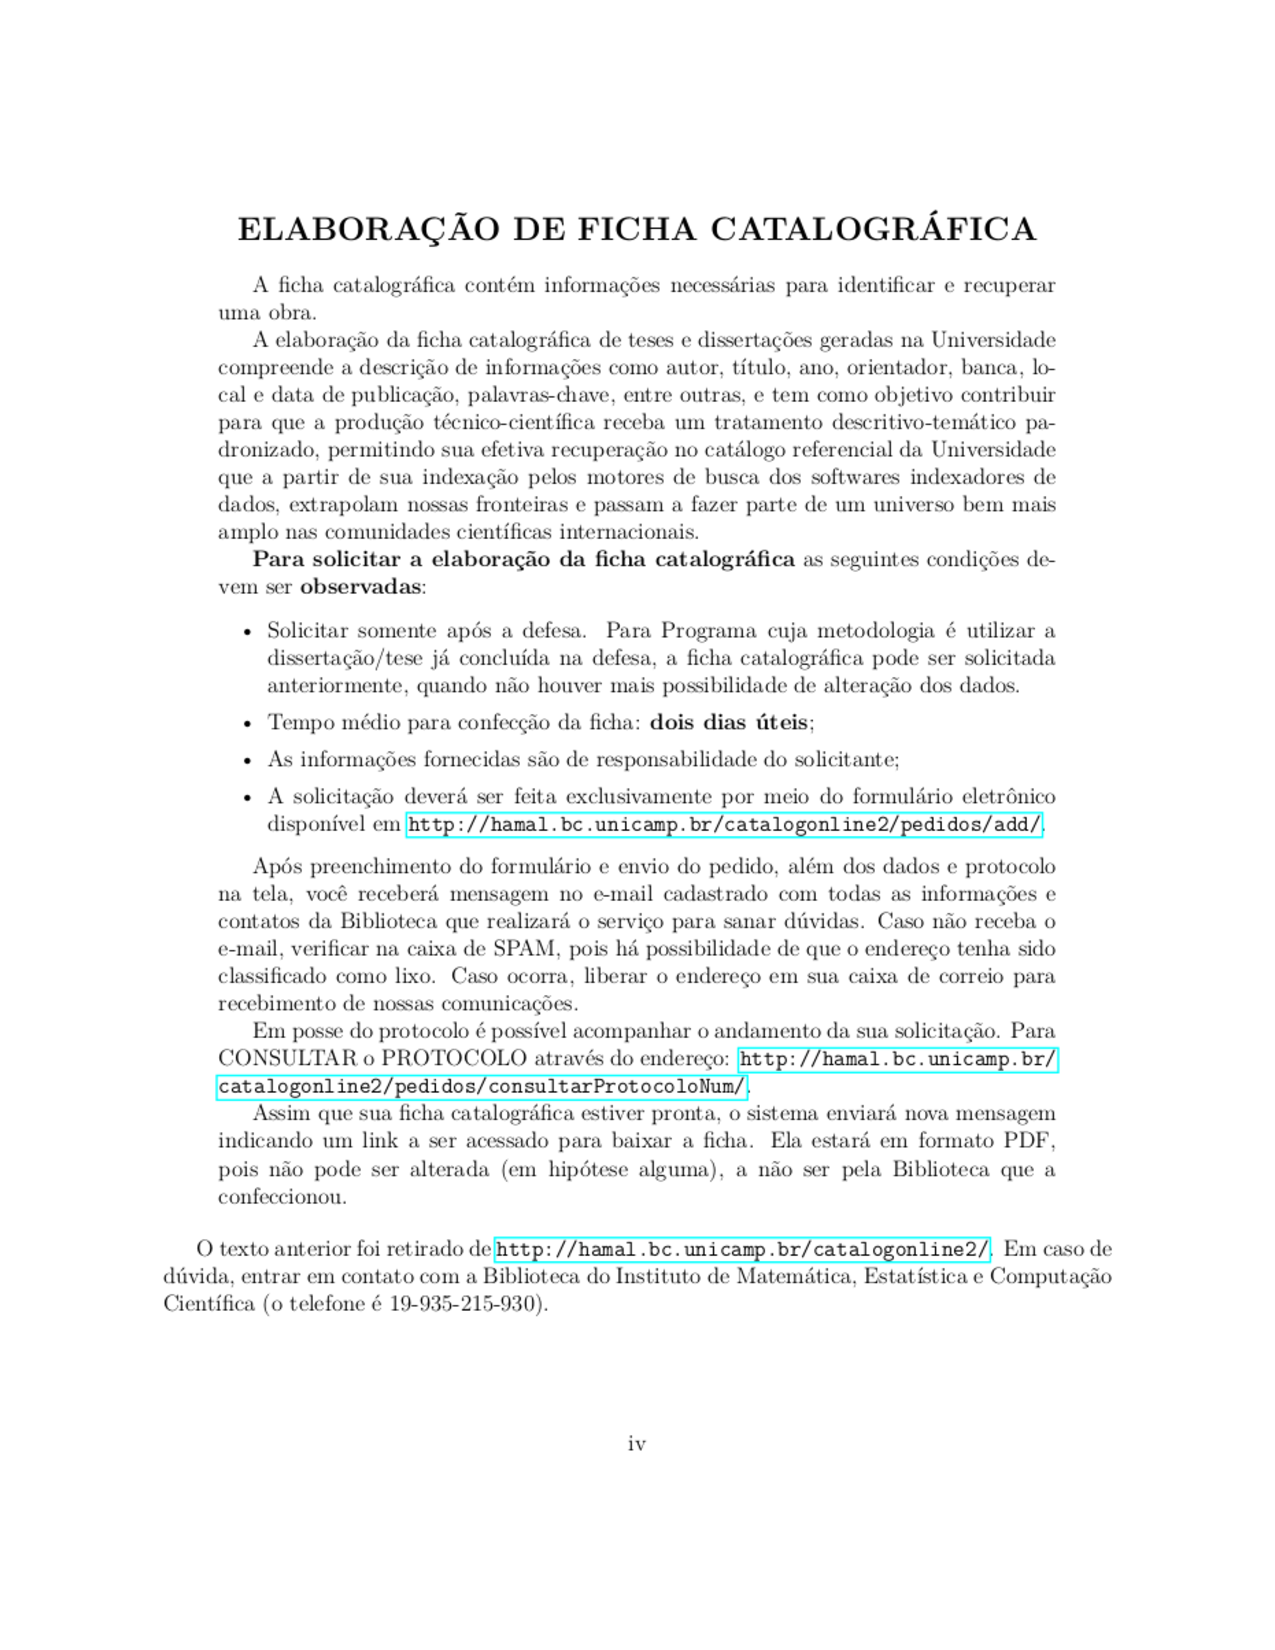
\includepdf{ficha-catalografica.pdf}
\end{fichacatalografica}
%==================================================================================================
%                                   FOLHA DE APROVAÇÃO
%==================================================================================================
% WARNING A folha de aprovação deve ser assinada pelos membros da banca apos a
% defesa.
% TODO Incluir folha de aprovação escaneada e alterar nome do arquivo.
% FIXME Substitua o arquivo folha-de-aprovacao.pdf por uma copia escaneada.
%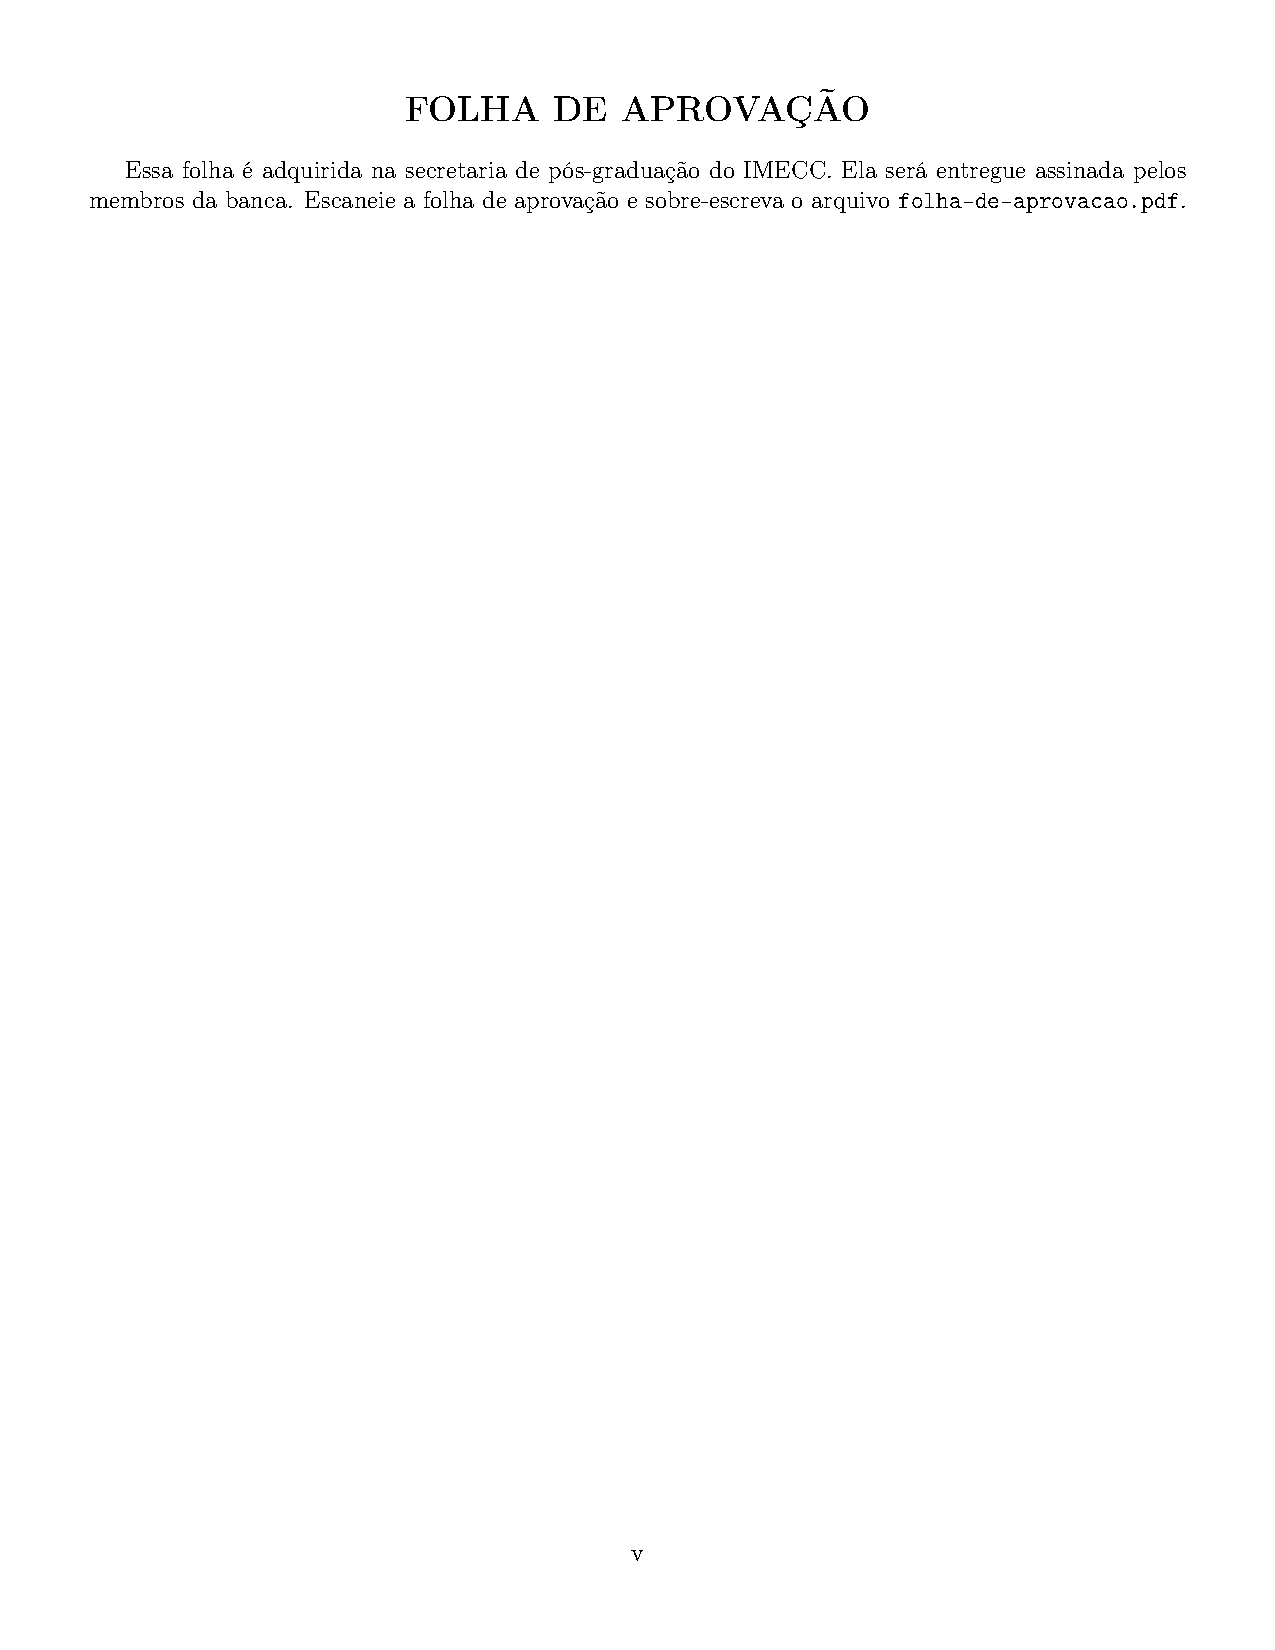
\includepdf{Dissertacao_folha-de-aprovacao}
	
	% --- Inserir folha de aprova\c{c}\~{a}o ---
	%\includepdf{folha_de_assinaturas_oficial.pdf}
	
	% Isto \'{e} um exemplo de Folha de aprova\c{c}\~{a}o, elemento obrigat\'{o}rio da NBR
	% 14724/2011 (se\c{c}\~{a}o 4.2.1.3). Voc\^{e} pode utilizar este modelo at\'{e} a aprova\c{c}\~{a}o
	% do trabalho. Ap\'{o}s isso, substitua todo o conte\'{u}do deste arquivo por uma
	% imagem da p\'{a}gina assinada pela banca com o comando abaixo:
	
	% --- Na vers\~{a}o final, exclua essas linhas e insira o \includepdf
%==================================================================================================
%                                   FOLHA DE ASSINATURAS
%==================================================================================================
\newpage
\vspace*{\fill}
\begin{center}
	\textsc{Inclua aqui a folha de assinaturas.}
\end{center}
\vspace*{\fill}
\newpage
% --- --- ---
%\includepdf[pagecommand={\thispagestyle{plain}}]{folha-assinaturas.pdf}	
%\cleardoublepage
\newpage

%==================================================================================================
%                                   DEDICATÓRIA
%==================================================================================================
% FIXME Se não for incluir a dedicatória, comentar a linha abaixo.
%\chapter*{\markboth{}{}}  % \markboth{}{} é utilizado para corrigir o cabeçalho.
\phantomsection
\addcontentsline{toc}{chapter}{Dedicatória}
\begin{center}

  % TODO Inserir a dedicatória aqui.
\end{center}
%
% ---

%% --- Dedicat\'{o}ria ---
\begin{dedicatoria}
	\vspace*{\fill}
	\centering
	\noindent
	\textit{Dedico esta tese \`{a} todo mundo.}
	\vspace*{\fill}
\end{dedicatoria}
%\setcounter{page}{}
%% ---
%==================================================================================================
%                                   AGRADECIMENTOS
%==================================================================================================
% FIXME Se não for incluir os agradecimentos, comentar a linha abaixo.
%\chapter*{Agradecimentos\markboth{Agradecimentos}{}}  % \markboth{}{} é utilizado para corrigir o cabeçalho.
\phantomsection
\addcontentsline{toc}{chapter}{Agradecimentos}

%% --- Agradecimentos ---
\begin{agradecimentos}
	Escreva seus agradecimentos.
	
	
	\lipsum[1-3]
\end{agradecimentos}

%

%==================================================================================================
%                                   RESUMOS E ABSTRACT
%==================================================================================================
\begin{resumo}

Insira seu resumo.

\lipsum[1]

\vspace{\onelineskip}

\noindent\textbf{Palavras-chaves}: palavra-chave 1; palavra-chave 2; palavra-chave 3.

\vspace{\onelineskip}
\vspace{\onelineskip}
\begin{otherlanguage*}{english}
	\begin{center}{\ABNTEXchapterfont\huge Abstract}\end{center}
	
	This thesis analyses the dynamics of household investment and the impacts of credit crunch using a Sraffian Supermultiplier Stock-Flow Consistent (SSM-SFC) model based on the U.S. economy (1980-2000). The first chapter presents a brief review of recent literature of heterodox growth models focusing on the neo-Kaleckian and sraffian supermultiplier models. The second chapter highlights stylezed facts for the American economy which support the idea that non‐capacity generating expenditures, mainly household investment, led the economic growth. In the third chapter, a SSM-SFC model with asset price bubbles is simulated to analyse the effects of some shocks such as  changes in income distribution, house prices dynamics,  and interest rate of loans.     
	
	\vspace{\onelineskip}
	
	\noindent\textbf{Keywords}: keyword 1; keyword 2; keyword 3. 
	
\end{otherlanguage*}
\end{resumo}
%==================================================================================================
%                                   EPÍGRAFE
%==================================================================================================

%% --- Ep\'{\i}grafe  ---
\begin{epigrafe}
	\vspace*{\fill}
	\begin{flushright}
		\textit{``Não está ao meu alcance criar uma sociedade ideal. Contudo, está ao meu alcance descrever o que, na sociedade existente, não é ideal para nenhuma espécie de existência humana em sociedade.''\\
			(Florestan Fernandes)}
	\end{flushright}
\end{epigrafe}
%\cleardoublepage
\newpage
%% ---

%==================================================================================================
%                                   ÍNDICE
%==================================================================================================
\tableofcontents*
%\cleardoublepage
\newpage
%
%
%
%==================================================================================================
%                                   LISTA DE ILUSTRAÇÕES
%==================================================================================================
\pdfbookmark[0]{\listfigurename}{lof}
\listoffigures*
\addcontentsline{toc}{chapter}{Lista de Ilustrações}
%\cleardoublepage
\newpage
%% ---
%
%==================================================================================================
%                                   LISTA DE TABELAS
%==================================================================================================
\pdfbookmark[0]{\listtablename}{lot}
\listoftables*
\addcontentsline{toc}{chapter}{Lista de Tabelas}
%\cleardoublepage
\newpage
%% ---
%
%==================================================================================================
%                                   LISTA DE VARIÁVEIS
%==================================================================================================
\chapter*{Lista de Variáveis\markboth{Lista de Variáveis}{}}  % \markboth{}{} é utilizado para corrigir o cabeçalho.

Listas de variáveis e parâmetros utilizadas no modelo SFC.

\section*{Variáveis endógenas}

\begin{description}
	\item[$C_w$] Consumo dos trabalhadores (induzido)	
	\item[$C_k$] Consumo dos capitalistas (autônomo)	
	\item[$FD$] Lucros distribuídos
	\item[$Fn$] Lucros líquidos
	\item[$FT$] Lucros totais
	\item[$FU$] Lucros retidos
	\item[$g_K$] Taxa de crescimento do estoque de capital
	\item[$g_{I_h}$] Taxa de crescimento do investimento residencial
	\item[$g_{Z}$] Taxa de crescimento dos gastos autônomos
	\item[$h$] Propensão marginal a investir (não-residencial)
	\item[$I_t$] Investimento total
	\item[$I_f$] Investimento das firmas
	\item[$I_h$] Investimento residencial (construção de novos imóveis)
	\item[$I_{hs}$] Investimento residencial (oferta)
	\item[$K_{HS}$] Estoque de imóveis (oferta)
	\item[$K_{HD}$] Estoque de imóveis (demanda)
	\item[$K_{f}$] Estoque de capital produtivo (firmas)
	\item[$K_{nom}$] Estoque de capital total (nominal)
	\item[$K$] Estoque de capital total (real)
	\item[$K_{k}$] Participação dos imóveis no estoque de capital % Rever
	\item[$L$] Empréstimo total
	\item[$L_f$] Empréstimo das firmas
	\item[$L_k$] Empréstimo aos capitalistas
	\item[$M$] Depósitos bancários (Moeda)
	\item[$MO$] Hipotecas
	\item[$NFW_b$] Riqueza financeira líquida dos bancos
	\item[$NFW_f$] Riqueza financeira líquida das firmas
	\item[$NFW_h$] Riqueza financeira líquida das famílias
	\item[$NFW_{hk}$] Riqueza financeira líquida das famílias capitalistas
	\item[$NFW_{hw}$] Riqueza financeira líquida das famílias trabalhadoras
	\item[$p_h$] Preço dos imóveis
	\item[$r_l$] Taxa de juros dos empréstimos das firmas
	\item[$r_{mo}$] Taxa de juros das hipotecas
	\item[$S_{hk}$] Poupança das famílias capitalistas
	\item[$S_{hw}$] Poupança das famílias trabalhadoras
	\item[$u$] Grau de utilização da capacidade
	\item[$V_b$] Riqueza líquida dos bancos
	\item[$V_f$] Riqueza líquida das firmas
	\item[$V_h$] Riqueza líquida das famílias
	\item[$V_{hk}$] Riqueza líquida das famílias capitalistas
	\item[$V_{hw}$] Riqueza líquida das famílias trabalhadoras
	\item[$W$] Salários
	\item[$Y$] Renda (PIB)
	\item[$YD$] Renda disponível das famílias
	\item[$YD_k$] Renda disponível das famílias capitalistas
	\item[$YD_w$] Renda disponível das famílias trabalhadoras
	\item[$Y_{FC}$] Produto potencial
	\item[$Z$] Gastos autônomos não criadores de capacidade
\end{description}


\section*{Variáveis exógenas}

\begin{description}
	\item[$\omega$] Participação dos salários na renda
	\item[$rm$] Taxa de juros dos depósitos bancários
	\item[$\sigma_l$] \textit{spread} dos empréstimos das firmas
	\item[$\sigma_{mo}$] \textit{spread} dos empréstimos das hipotecas
	\item[$u_N$] Grau de utilização normal
	\item[$v$] Relação técnica capital-produto
	\item[$\pi$] Inflação de ativos (imóveis)
	\item[$R$] Participação do consumo financiado por crédito nos gastos autônomos não criadores de capacidade produtiva
\end{description}



\section*{Parâmetros}

\begin{description}
	\item[$\alpha$] Propensão marginal a consumir a partir dos salários
	\item[$\gamma_F$] Participação dos lucros não distribuídos nos lucros totais
	\item[$\gamma_u$] Parâmetro de ajustamento da propensão marginal a investir
	\item[$\phi_0$] Componente autônomo do investimento residencial
	\item[$\phi_1$] Sensibilidade do investimento a taxa própria de juros
\end{description}

\addcontentsline{toc}{chapter}{Lista de Variáveis}

%==================================================================================================
%                                   ABREVIAÇÕES
%==================================================================================================
% FIXME Comentar a linha abaixo de não for apresentar as
% abreviações e siglas utilizadas.
\chapter*{Lista de Abreviaturas e Siglas\markboth{Lista de Abreviaturas e Siglas}{}}  % \markboth{}{} é utilizado para corrigir o cabeçalho.

\addcontentsline{toc}{chapter}{Lista de Abreviaturas e Siglas}
%\cleardoublepage
\newpage
%
%==================================================================================================
%                                   SÍMBOLOS
%==================================================================================================
% FIXME Comentar a linha abaixo se não for apresentar os
% símbolos utilizados.
%\input{Dissertacao_simbolos}
%==================================================================================================
%                                   ALGORITMOS
%==================================================================================================
% FIXME Comentar a linha abaixo se não desejar listar os algoritmos
% apresentados.
%\listofalgorithms
%==================================================================================================
%                                   CÓDIGO
%==================================================================================================
% FIXME Comentar a linha abaixo se não desejar listar os trechos de código
% apresentados.
%\lstlistoflistings
%==================================================================================================
%                                   NUMERAÇÃO
%==================================================================================================
% As paginas com o conteúdo da tese são numeradas com algoritmos arábicos.
%\mainmatter
% TODO Corrigir numeração romana antes da dissertação
%
%==================================================================================================
%                                   CAPÍTULOS DA DISSERTAÇÃO
%==================================================================================================
% ---- ELEMENTOS TEXTUAIS ----
\mainmatter
\cleardoublepage\pagenumbering{arabic}
\setcounter{page}{14}
\chapter{Da instabilidade de Harrod à estabilidade fundamental}

\epigraph{Is it not rather odd when dealing with ``long-run problems'' to start with the assumption that all firms are always working below capacity?}{Keynes to Kalecki}


Este capítulo faz uma breve revisão da literatura dos modelos de crescimento liderados pela demanda. Apresenta a instabilidade harrodiana para então avaliar a forma que essa problemática é tratada pelas teorias heterodoxas.
Ao final desta exposição, serão privilegiados aqueles modelos que atendem o princípio da demanda efetiva (PDE) no curto-, médio- e longo-prazo. Em outras palavras, o PDE bem como alguns fatos estilizados serão utilizados como critério de seleção para eleger um modelo a ser examinado nos capítulos seguintes.

%TODO Reescrever estrutura do capítulo após modificações

Para atender esses objetivos, a seção \ref{SecHarrod} explicita a instabilidade de Harrod e as respostas dos modelos de Cambridge, neo-/pós-Kaleckianos e Supermultiplicador Sraffiano. Compreendidas tais propostas, mapeia-se o debate sobre a convergência do grau de utilização ao nível normal e as implicações sobre os paradoxos dos custos e da parcimônia. Na seção \ref{Literatura} é feito um levantamento bibliográfico sobre os modelos de crescimento com gastos autônomos não criadores de capacidade. Por fim, a seção \ref{Concl1} contém as considerações finais e elege o modelo a ser utilizado nos capítulos seguintes.





\section{Instabilidade de Harrod: princípios e provocações}\label{SecHarrod}

%=============== Inicio: Ligação Harrod ============

As origens da teoria macrodinâmica devem, em grande parte, às contribuições de \textcite{harrod_essay_1939} em que extrapola o principio da demanda efetiva formulado por \textcite{keynes_general_1936} para uma economia em crescimento. Tal modelo impôs importantes questões: Existe estabilidade do crescimento no longo pra\-zo? É possível equacionar o crescimento da demanda com o crescimento da capacidade produtiva? Se sim, qual variável acomoda essa adequação? A capacidade produtiva se ajusta à demanda ou o inverso? Os modelos de Cambridge, Oxford e do tipo supermultiplicador responderam essas provocações de formas distintas e serão analisados ao longo desta seção.

Para evitar redundâncias, são apresentadas as hipóteses que permeiam as famílias de modelos aqui avaliadas. 
A presente exposição prioriza a parcimônia e, portanto, trata-se de uma economia sem relações externas e sem governo em que tanto progresso tecnológico quanto retornos crescentes de escala estão ausentes. Além do PDE, o que torna os modelos em questão consistentes é o abandono da substitutibilidade entre capital e trabalho e, portanto, adota-se uma função de produção \textit{à la} Leontief em que existem dois produtos potenciais: plena capacidade ($Y_K$) e pleno emprego ($Y_L$) de modo que o produto potencial ($Y_{FC}$) é determinado por:

\begin{equation}
    Y_{FC} = \min (Y_K, Y_L)
\end{equation}
Seguindo a literatura, em que o estoque capital ($K$) é o fator escasso,
\begin{equation}
\label{Oferta}
    Y_{FC} = Y_K = \frac{1}{v}K_{t-1}
\end{equation}
em que $v$ é a relação técnica capital-produto. 


Considerando as hipóteses anteriores, a determinação do produto pelos componentes da demanda é obtida pela soma do consumo e investimento. Como será visto adiante, a distinção entre os modelos recairá sobre a autonomia (completa, parcial ou nula) do investimento das firmas e a existência de gastos autônomos não criadores de capacidade produtiva (denotados por $Z$). De modo a expor o problema deixado por \textcite{harrod_essay_1939}, supõe-se que o consumo é completamente induzido e que não existem gastos ``improdutivos'' ($Z=0$). Assim, o produto determinado pela demanda é dado pelo multiplicador:

\begin{equation}
\label{Demanda}
Y = \frac{I}{s}
\end{equation}
em que $s$ é a propensão marginal a poupar e $I$ é o investimento.
O princípio acelerador --- neste caso, acelerador rígido\footnote{Para o caso com acelerador rígido e uma dada propensão marginal a consumir ($c = 1-s$), o consumo é induzido, tem-se:
	$$
	Y = c\cdot Y + v\cdot \Delta Y
	$$
	rearranjando, obtém-se:
	$$
	\frac{\Delta Y}{Y} = g = \frac{1 - c}{v} = \frac{s}{v}
	$$
	que equivale à equação fundamental de Harrod.
} ---, por sua vez, estabelece que a determinação do investimento decorre das alterações na demanda (efetiva), ou seja, decorre do princípio de ajuste do estoque de capital:
$$
K = v\cdot Y
$$
\begin{equation}
\Delta K = I = \overline{v}\Delta Y
\end{equation}


%Tomando o modelo mais genérico, em que consumo é parcialmente induzido ($C$), o investimento criador de capacidade produtiva ao setor privado ($I$) possui uma parcela autônoma ($\overline I$) e outra induzida e os gasto autônomos são não nulos ($Z > 0$), obtém-se a determinação do produto pelos componentes da demanda:
%\begin{equation}
%\label{Demanda}
%    Y = C + I + Z
%\end{equation}
A questão que permeia os modelos analisados são as condições para que exista um crescimento equilibrado da demanda (Eq. \ref{Demanda}) e da capacidade produtiva (Eq. \ref{Oferta}). 
Argumenta-se que a junção destes dois conceitos permite tratar o Princípio da Demanda Efetiva de forma dinâmica e que esta é a essência do modelo de Harrod cuja Equação fundamental pode ser deduzida da identidade entre poupança ($S$) e investimento:

$$
s\cdot Y = S \equiv I
$$
Neste ponto, fica evidente que neste modelo a propensão marginal à poupar ($s$) é igual a propensão média à poupar ($S/Y$) na ausência dos gastos autônomos não criadores de capacidade\footnote{As implicações desta igualdade será analisada mais detidamente ao tratar do supermultiplicador sraffiano.}. Em seguida, basta normalizar esta identidade pelo estoque de capital,
$$
\frac{I}{K} = s\frac{Y}{K}
$$
$$
\frac{I}{K} = s\frac{Y}{v\cdot Y_K}
$$
\begin{equation}
    g_K = \frac{s}{v}u
\end{equation}
em que $g_K$ é a taxa de acumulação e $u$ é o grau de utilização da capacidade definido por:
$$
u = \frac{Y}{Y_{FC}}
$$
e sua taxa de crescimento pode ser dada por
$$
g_u = g_Y - g_{Y_{FC}}
$$
Além disso, para que o grau de utilização se estabilize, é preciso que, no \textit{steady state}, produto e capacidade produtiva cresçam a uma mesma taxa. Com isso, obtém-se a equação fundamental de Harrod:

\begin{equation}
    \label{Fundamental}
    g_w = \frac{s}{v}u_N
\end{equation}
em que $g_w$ é a taxa de crescimento que garante que a demanda e capacidade produtiva cresçam dinamicamente equilibradas. Além disso, pelo grau de utilização estar em seu nível desejado ($u_N$), esta taxa corresponde àquela que os empresários estariam satisfeitos e não haveria razões para alterar seu comportamento e/ou planos de investimento. 

Neste modelo, quando a taxa efetiva é maior (menor) que a taxa garantida, o grau de utilização da capacidade é maior (menor) que o planejado. Nesse caso, as firmas buscam ampliar (reduzir) sua capacidade produtiva com o objetivo que o grau efetivo de utilização da capacidade convirja ao normal. O aumento (redução) da taxa de crescimento do investimento tem um impacto imediato na taxa de crescimento da
economia e, apenas de depois de alguma defasagem, na taxa de crescimento do estoque de capital. O resultado, portanto, é um grau de utilização da capacidade ainda mais distante do planejado. O problema é justamente que, dado o acelerador rígido, o mecanismo de ajuste do modelo leva a economia cada vez mais distante da sua posição de \textit{steady-state}. A esse processo Harrod (1939) denomina de instabilidade fundamental. Em outras palavras, quando o grau de utilização efetivo se difere do normal ($u\neq u_N$),  a taxa de crescimento efetiva é diferente da garantida e esta diferença se acentua ao longo tempo


%a taxa de crescimento efetiva se afasta da taxa desejada em função da reação do investimento à variações no nível de atividade. Seguindo o princípio acelerador nos moldes de \textcite{harrod_essay_1939}, a resposta a uma sobreutilização da capacidade ($u>1$) é o aumento da taxa de acumulação que, pelo efeito multiplicador gera  demanda, reforçando o mecanismo de descolamento, para então ampliar a capacidade produtiva \cite[p.~12]{serrano_trouble_2017}.  No entanto, uma vez que essas são diferentes, não há um mecanismo de convergência entre elas.


% =============== Instabilidade fundamental Serrano et all ==========

Tendo em vista que neste modelo o princípio do acelerador é o principal determinante da trajetória, \textcite[p.~26--28]{harrod_essay_1939} procura reduzir tais efeitos incluindo frações do investimento que não estão diretamente relacionados com a renda corrente. Tal constatação introduz a possibilidade de que exista um componente autônomo do investimento que não é afetado pelo mecanismo de ajuste do estoque de capital no longo prazo e, portanto, permite que a instabilidade harrodiana seja amenizada:

\begin{citacao}
Now, it is probably the case that in any period not the whole of the new capital is destined to look after the increment of output of consumers' goods. There may be  long-range plans of capital development or a transformation  of the method of  producing  the pre-existent level of output. \cite[p.~17]{harrod_essay_1939}
\end{citacao}
adiante
\begin{citacao}
The force  of this  argument [Princípio da instabilidade], however, is somewhat \textbf{weakened} when long-range  capital outlay is taken into account.
\cite[p.~26, grifos adicionados]{harrod_essay_1939}
\end{citacao}
Tal possibilidade, como será discutido adiante, sugere que a instabilidade harrodiana não decorre do princípio de ajuste do estoque de capital, mas sim, da especificação da propensão marginal (e média) a poupar e da rigidez do acelerador. Isso implica que um modelo em que o investimento é induzido pelo princípio do ajuste de estoque de capital não é necessariamente instável.

Uma observação importante é que apesar de \textcite[p.~23]{harrod_essay_1939} afirmar que existe uma única taxa de crescimento garantida, \textcite[p.~83]{robinson_model_1962} alerta que isso não implica que o investimento % Usado como sinônimo de crescimento
deve se adequar a propensão marginal a poupar determinada \textit{a priori}. Argumenta que os modelos liderados pela demanda devem ser avaliados pelas respectivas formas de induzir o investimento uma vez que o Princípio da Demanda Efetiva é o denominador comum entre eles. Portanto, dadas as hipóteses compartilhadas, os respectivos  fechamentos\footnote{Entende-se por fechamento como variável que assume valores economicamente relevantes de tal forma a tornar determinada relação (e.g. taxa de lucro) válida. Em outras palavras, trata-se da última variável que é resolvida endogenamente. Desse modo, dizer que o fechamento de um modelo é estabelecido por uma variável (digamos, $j$) implica dizer que $j$ é endógena. Além disso, por se tratar de um modelo generalizante de crescimento, dizer que distribuição de renda é exógena significa em ausência de simultaneidade entre distribuição e acumulação.} permitem uma análise comparativa e por isso será adotada adiante. Para isso, a equação fundamental de Harrod é rearranjada para explicitar algumas relações.


As hipóteses enunciadas anteriormente são preservadas para evitar repetições desnecessárias. Adicionalmente, inclui-se a possibilidade de existência de gastos autônomos não criadores de capacidade produtiva para garantir a comparação entre os modelos analisados. Com essa hipótese adicional, a propensão média à poupar torna-se uma função tanto dos gastos autônomos ($Z$) quanto do produto:

\begin{equation}
\label{Poupanca_Super}
    \frac{S}{Y} = s - \frac{Z}{Y}
\end{equation}
Seguindo a notação de \textcite{serrano_sraffian_1995}, seja $f$ a relação entre propensão média e marginal a poupar
$$
f = \frac{\frac{S}{Y}}{s}
$$
de modo que será igual a unidade quando forem idênticas. Nesses termos, a equação \ref{Fundamental} pode ser reescrita como:

\begin{equation}
 \label{EqGeral}   
g_K = g_w = f\frac{s\cdot u_N}{\overline v}
\end{equation}

A equação acima permite comparar os modelos\footnote{Por padrão, as variáveis/parâmetros exógenos serão, $j$ por exemplo, serão denotados como $\overline j$.} analisados de modo a destacar a variável que garanta, 
$$
g_K = g
$$
a começar pelo de Cambridge.

\subsubsection{Modelo de Cambridge}

%TODO Mais contexto

O modelo de Cambridge\footnote{Para uma análise mais detalhada das origens e extensões do modelo de Cambridge, ver \textcite{baranzini_cambridge_2013}.} tinha entre seus objetivos estender as implicações do princípio da demanda efetiva para o longo prazo sem que, para isso, incorresse em um aparato marginalista\footnote{
	Como destaca \textcite[p.~127--133]{davidson_accumulation_1978}, tais autores estavam preocupados em analisar economias com taxas de crescimento equilibradas --- e não na transição entre diferentes trajetórias de crescimento --- em condições normais (``tranquilas'', sem distúrbios persistentes) na ausência de frustração de expectativas.
} \cites{kaldor_alternative_1955}{kaldor_model_1957}{robinson_model_1962}{pasinetti_rate_1962}. 
Para tanto, lançam mão --- explícita e implicitamente --- das seguintes hipóteses adicionais: 
	(i) os preços são mais flexíveis do que os salários nominais no longo prazo; 
	(ii) economia opera ao nível normal da capacidade\footnote{
		Na versão de \textcite{robinson_model_1962} trata-se de plena capacidade enquanto na de \textcite{kaldor_alternative_1955} a economia opera sob pleno-emprego.
	}; 
	(iii) investimento é autônomo\footnote{Além de ser autônomo, depende da taxa de lucro esperada na versão de \textcite{robinson_model_1962}.} e esta autonomia está associada aos  \textit{animal spirits}\footnote{Esse componente autônomo do investimento produtivo será levado adiante pelos modelos Kaleckianos.} e;
	(iv) as propensões marginais a poupar das classes sociais são distintas por conta da propensão marginal a consumir dos trabalhadores ser maior que a dos capitalistas. 
	
%Apresentadas as hipóteses, resta analisar como tais autores lidaram com o problema levantado por Harrod. \textcite{robinson_model_1962} afirma que quando a composição do estoque de capital está adequada com a taxa de crescimento desejada e quando as expectativas das firmas estão de acordo com o desempenho corrente da economia, então o modelo está sob uma taxa de equilíbrio interna. Já \textcite{kaldor_alternative_1955}\footnote{
%	\textcite{kaldor_model_1957}, por outro lado, afirma que a metodologia por ele utilizada se assemelha à de \textcite{harrod_essay_1939}, mas tem diferenças, tais como: (i) Crescimento é limitado pela disponibilidade de recursos e não pela insuficiência de demanda efetiva; (ii) Não distingue mudanças técnicas decorrentes de maior acumulação de capital daquelas resultantes de inovações; (iii) Estoque de capital em termos reais é medido pela quantidade de ferro incorporada; (iv) O crescimento econômico decorre tanto da rapidez na absorção de mudanças tecnológicas quanto da propensão à investir; (v) Autoridade monetária é passiva de modo que a taxa de juros de longo prazo é igual à taxa de lucro.
%} supõe que o multiplicador keynesiano determinaria o nível de produto no curto-prazo.
A primeira diferença em relação ao modelo de Harrod é o investimento tratado como autônomo, com isso eliminando a origem da instabilidade harrodiana decorrente --- na leitura de Cambridge --- do investimento reagir ao grau de utilização da capacidade.
Além disso, esses autores assumem uma estrutura da economia \textit{à la} \textcite{kalecki_theory_1954}, explicitando as classes sociais. Os trabalhadores, por hipótese, não poupam, logo toda a poupança é feita pelos capitalistas

$$
S = s_p\cdot FT
$$
em que $s_p$ é a propensão marginal a poupar dos capitalistas a partir dos lucros e; $FT$ são os lucros totais. Partindo da decomposição de \textcite{weisskopf_marxian_1979}, é possível escrever a taxa de lucro nos seguintes termos:
$$
r = \frac{FT}{K} = \frac{FT}{Y}\frac{Y}{Y_{FC}}\frac{Y_{FC}}{K}
$$ 
\begin{equation}
\label{LucroCambridge}
r = \frac{(1-\omega)\cdot u}{v}
\end{equation}
seguindo \textcite{serrano_trouble_2017} e retomando a hipótese de plena utilização do capital, temos
$$
g = \frac{I}{K} 
$$
$$
\frac{I}{K} = \frac{S}{K}\frac{Y}{Y}\frac{Y_{fc}}{Y_{fc}} = s_p\frac{FT}{K}\frac{Y}{Y}\frac{Y_{fc}}{Y_{fc}}
$$
Alterando a equação \ref{EqGeral}, 
\begin{equation}
%\label{Sintetica}
g = s_p\cdot \frac{(1-\omega)\cdot u}{v}
\end{equation}
em que $\omega$ é a participação dos salários na renda ($\omega = W/Y$) e $r$ é a taxa efetiva de lucro enquanto a Equação \ref{EqCambridge} é a famosa equação de Cambridge\footnote{
	Para uma exposição de seus antecedentes e implicações, ver \textcite{bortis_notes_1993}.
}.

\begin{equation}
\label{EqCambridge}
g = s_p\cdot r
\end{equation}

\begin{equation}
\label{Cambridge}
(1-\omega) = \frac{g\cdot v}{s_p}
\end{equation}


As equações acima evidenciam que neste modelo a distribuição funcional da renda é a variável de fechamento  e apresenta uma relação implícita e simultânea com a taxa de lucro. Como consequência, os lucros são positivamente determinados pela acumulação\footnote{
	Posteriormente, parte da literatura tem associado esse resultado aos microfundamentos decorrentes da teoria gerencialista da firma em que maiores taxas de crescimento --- como visto, determinadas pelo investimento autônomo --- requerem maiores taxas de lucro, implicando maiores \textit{mark-ups} e uma barreira inflacionária \cite[p.~353]{lavoie_post-keynesian_2015}
}\footnote{Parte considerável das críticas dizem respeito à função de poupança nesta família de modelos uma vez que está associada com os lucros retidos das firmas. Para maiores detalhes, ver  \textcites[Seção III]{skott_kaldoriansaving_1981}{marglin_foundation_1984}{skott_kaldors_1989}.}. 
%MAIS REFERÊNCIAS
Em outras palavras, no curto prazo --- preços e salários rígidos --- o produto é determinado pelo investimento (autônomo) via multiplicador enquanto no longo prazo o nível de produto é igual ao seu potencial ($Y = Y_{FC}, \,u=1$) enquanto os preços são flexíveis\footnote{
	Neste ponto vale lembrar as distinções entre os principais autores desta família de modelos que, por sua vez, não comprometem o grau de generalidade da análise aqui realizada. 
	%Enquanto \textcite[5--6]{kaldor_alternative_1955} e \textcite{pasinetti_rate_1962} assumiam que o nível de investimento seria suficiente, no longo prazo, para garantir o pleno-emprego;.
	A título de exemplo, \textcite{robinson_model_1962} pressupunha --- na ausência de uma barreira inflacionária --- uma política monetária acomodatícia de modo que não existiriam restrições ao financiamento do investimento e, assim, a economia operaria em plena utilização da capacidade.
}. Assim, mudanças na taxa de crescimento do gasto autônomo (investimento) teriam como contrapartida variação do nível de preços e mudanças na distribuição\footnote{Para uma crítica da relação entre grau de utilização e preços normais, ver \textcite{ciccone_2017}.}. 

Portanto, no modelo de Cambrigde, existe uma relação simultânea e necessária entre crescimento e distribuição de modo que ser resumido nos seguintes termos:

\begin{citacao}
The main message of the Cambridge
equation is that the warranted growth rate is determined by the rate of capital
accumulation gk that results from the investment decisions of entrepreneurs; this
determines the long-period (or normal) income distribution, which thereby
becomes endogenous and subordinated to the rate of accumulation \cite[p.~158]{cesaratto_neo-kaleckian_2015}
\end{citacao}
Desse modo, obtém-se uma relação positiva entre poupança e crescimento no longo prazo ou ainda uma relação negativa entre salários reais e taxa lucros (como explicitado na Eq. \ref{LucroCambridge}). Consequentemente, para a garantir o equilíbrio entre demanda e capacidade produtiva associado a uma maior taxa de crescimento é necessário que uma parcela menor da renda seja destinada ao consumo. A importância de explicitar esta causalidade em termos do consumo é que destaca a importância do mecanismo de preços no modelo e a respectiva resolução da instabilidade de Harrod. Como mencionado anteriormente, os preços são mais flexíveis do que os salários por hipótese. Assim, se a taxa crescimento da economia estiver acima da taxa garantida, instaura-se um aumento dos preços acima dos salários e opera-se um mecanismo de poupança forçada. O resultado é uma redução dos salários reais e, por definição, aumento da participação dos lucros na renda.  Neste modelo, portanto, é justamente a mudança na distribuição funcional da renda, e consequentemente a propensão marginal a poupar da economia, que promove o ajuste da taxa garantida para a taxa efetiva de crescimento assegurando a estabilidade do modelo.

Apesar do modelo de Cambridge recorrer a relação entre acumulação e distribuição como fechamento, argumenta-se aqui que a adequação da capacidade
produtiva à demanda não precisa lançar mão de tais hipóteses.
Não apenas isso, mas tanto os salários reais quanto a taxa de lucro não são \textit{necessariamente} determinados pelo investimento

\begin{citacao}
\textit{When it is
capacity that adjusts to aggregate output, rather than output to
capacity, the disappearance of excess capacity in the long period is
the result of a low aggregate demand, and cannot therefore have
acted as a constraint upon it, imposing a choice between consumption
and investment and, hence, between wages and profits} \cite[p.~50]{halevi_notes_2014}.
\end{citacao}
Desse modo, a igualdade entre poupança e investimento não se dá por variações no produto dada a inelasticidade --- por hipótese --- do produto potencial em relação a demanda.
Se, por outro lado, a elasticidade de ajustamento da capacidade produtiva a demanda for maior no longo prazo --- como argumenta \textcite[p.~62--3]{halevi_notes_2014} ---, o equilíbrio dinâmico entre ambas não precisa supor a endogeneidade da distribuição\footnote{\textcite[p.~158]{cesaratto_neo-kaleckian_2015}, por sua vez, destaca a falta de robustez na relação entre taxas de crescimento mais elevadas e mudanças na distribuição de renda a favor dos lucros.
	Tais limitações do modelo de Cambridge não devem ser entendidas como uma impossibilidade do crescimento ser \textit{demand-led} no longo prazo.}:

\begin{citacao}
	\textit{The elasticity that a capitalist economy is thus shown to have in
	reacting to incentives for a more rapid growth by bringing about
	additional productive capacity, or, symmetrically, by eliminating
	excess capacity and erasing the visible traces of the losses in output
	due to a low such incentive, should have already made clear that no
	necessity exists for a change in the real wage, and in the associated
	normal rate of profits, in order to generate (eliminate) the savings
	corresponding to any increased (decreased) demand for investment} \cite[p.~53]{halevi_notes_2014}
\end{citacao}
 

Na tentativa de responder à instabilidade de Harrod, outra parcela da literatura também discorda --- por meio de hipóteses sobre a estrutura de mercado --- da hipótese de endogeneidade da distribuição de renda.
%TODO Sinônimo de abandonar
A título de exemplo, \textcite{steindl_stagnation_1979} afirma que em seu livro de 1952 \cite{steindl_maturity_1952} possuía um raciocínio semelhante ao de Kaldor para o caso de estrutura de mercado competitiva em que tanto as taxas de lucro quanto o grau de utilização estariam em seu nível normal no longo prazo. No entanto, quando revisita essa ideia \cite{steindl_stagnation_1979}, afirma que tal análise da distribuição não é adequada para uma economia oligopolizada. Esta proposta será analisada na seção seguinte.

\begin{comment}
DESCARTADOS

\begin{equation}
\frac{I}{K} = g = \gamma + \gamma_r r
\end{equation}
Esse raciocínio pode ser traduzido em termos da equação \ref{Sintetica}\footnote{A versão proposta por \textcite{pasinetti_rate_1962} explicita as condições de \textit{stedy state} em que a taxa de juros e lucros precisam ser iguais no longo prazo. \textcite[p.~101]{kurz_post-keynesian_2010} destacam que a função poupança de Kaldor só é possível no longo prazo se a taxa de juros não exceder a taxa de lucros. Além disso, a exclusão da propensão marginal à poupar dos trabalhadores é decorrência do ``Teorema de Pasinetti'' em que a taxa de lucro independe da poupança dos trabalhadores.
}:

\begin{equation}
\label{Cambridge_Parcial}
\gamma + \gamma_r r = \mybox{$g = g_K$} =  f\frac{s_k\cdot u_N}{\overline v}
\end{equation}
Adiante, decompõe-se a taxa de lucro ($r$) nos termos de \textcite{weisskopf_marxian_1979}:
$$
r = \frac{P}{K} = \frac{P}{Y}\frac{Y}{Y_{FC}}\frac{Y_{FC}}{K}
$$
em que $P$ é a massa de lucros e $\omega$ o \textit{wage-share}. Como a relação capital-produto é considerada constante, a taxa de lucro depende simultaneamente do grau de utilização e distribuição de renda:
\begin{equation}
\label{Decomposicao_Lucro}
r = \frac{(1-\omega)\cdot u}{\overline v}  
\end{equation}
Substituindo a equação \ref{Decomposicao_Lucro} na \ref{Cambridge_Parcial}, obtém-se

$$
\gamma + \gamma_r \frac{(1-\omega)\cdot u}{\overline v} = \mybox{$g = g_K$} =  f\frac{s\cdot u}{\overline v}
$$


No modelo de Cambridge, a propensão marginal a poupar é definida exogenamente e é idêntica a propensão média, logo, $f=1$. Além disso, o grau de utilização converge ao normal e, portanto, não assume quaisquer valores necessários para garantir a igualdade entre demanda e capacidade produtiva e uma vez constante não pode ser a variável de fechamento. Por fim, supondo que o componente autônomo do investimento seja constante, isto é, $\gamma = \overline \gamma$ e isolando as variáveis endógenas restantes,

$$
\gamma_r \frac{(1-\omega)\cdot u}{\overline v} =   \frac{\overline s\cdot \overline u_N}{\overline v} - \gamma
$$

$$
\frac{(1-\omega)\cdot u}{\overline v} =   \left(\frac{\overline s\cdot \overline u_N}{\overline v} - \gamma\right)\frac{1}{\gamma_r}
$$

$$
(1-\omega) =   \left(\frac{\overline s\cdot \overline u_N}{\overline v} - \gamma\right)\frac{\overline v}{\overline \gamma_r \cdot \overline u_N}
$$

\begin{equation}
\label{Cambridge}
\therefore (1-\omega) = \frac{1}{\overline\gamma_r}\left(\overline s - \frac{\overline\gamma\cdot\overline v}{\overline u_N}\right)
\end{equation}

%Em linha com a formalização de \textcite[p.~347-59]{lavoie_post-keynesian_2015}, o raciocínio acima é estendido para a determinação da taxa de acumulação ($g_K$) que depende positivamente ($\gamma_r$) da taxa de lucro ($r$) e dos \textit{animal spirits} ($\gamma$)\footnote{Dentre os critérios para adequar um modelo, \textcite{robinson_model_1962} escolhe aquele que é compatível com os determinantes do comportamento humano em uma economia capitalista (\textit{animal spirit}). Além disso, a autora realça algumas características que considera fundamental em uma economia capitalista, tais como: produção é organizada por firmas (economia monetária de produção) e o consumo é destinado às famílias que, por sua vez, podem ser rentistas ou trabalhadoras. Alguns dos elementos citados anteriormente comporiam o centro da teoria pós-Keynesiana e que mereceriam uma análise mais detalhada. No entanto, dados os objetivos desta investigação, a ênfase recairá sobre a importância da autonomia do investimento.}:



\begin{citacao}
\textit{
In sum then, both Robinson and Kaldor-Pasinetti rely on	income redistribution via profit margins relative to money wages at a given level of employment to adjust when short-period entrepreneurial sales forecasts are proved incorrect,
while in The General Theory, Keynes suggested that changes in the level of employment were the primary short-period adjustment mechanism, with income distribution playing a less important role.	
} \cite[p.~127]{davidson_accumulation_1978}
\end{citacao}
Além disso, não são verificados os resultados decorrentes da teoria gerencialista da firma associados a essa teoria.
Tal microfundamentação implica na flexibilização dos preços e das margens de lucro dadas mudanças na demanda agregada que não é razoável seja no nível micro ou macroeconômico  e, portanto, deve ser rejeitada
\footnote{Para maiores detalhes, ver discussão em \textcites{ciccone_2017}[p.~104--5, n. 17]{serrano_teoria_1988}.}\footnote{
Outro tipo de crítica pode ser visto em \textcite[p.~127]{davidson_accumulation_1978} em que o autor realça a incompatibilidade com as implicações de uma economia monetária de produção:
\begin{citacao}

[I]t is an essential characteristic of a monetary economy that offer
prices and money wages should have short-period stickiness
and hence employment levels \textit{must} be more adjustable to disequilibrium conditions. Hence, these neo-keynesian models
will be seen to be deficient in terms of their discussions of
monetary aspects.
\end{citacao}
que, no entanto, não desqualifica a contribuição desses autores como pontua Davidson logo em seguida:

\begin{citacao}
Nevertheless, the authors of these models
recognised the limitations of their efforts and have continually
stressed that their analyses are basically concerned with long-run steady rates of equilibrium growth.
\end{citacao}
}. \textcite[p.~158]{cesaratto_neo-kaleckian_2015}, por sua vez, destaca a falta de robustez na relação entre taxas de crescimento mais elevadas e mudanças na distribuição de renda a favor dos lucros.
Tais limitações do modelo de Cambridge não devem ser entendidas como uma impossibilidade do crescimento ser \textit{demand-led} no longo prazo. Argumenta-se aqui que a adequação da capacidade produtiva à demanda não precisa lançar mão de tais hipóteses.
\end{comment}


\subsubsection{Modelo(s) kaleckiano(s)}

No pós-segunda guerra, parte da literatura tem dado ênfase para 
as implicações de uma tendência à estagnação secular \cite{setterfield_distribution_2002}.
Seguindo as contribuições de Kalecki, \textcite{steindl_maturity_1952} argumenta que tais economias --- ditas maduras --- possuem estruturas de mercado oligopolistas de modo que as firmas não realizam o ajuste entre demanda e capacidade produtiva via preço e, como consequência, o fechamento não poderia ser por meio da distribuição.
Dito isso, \textcite{steindl_stagnation_1979} afirma que na ausência de políticas expansionistas, de superávits na balança comercial e com a redução do consumo,  tais economias tenderiam a uma estagnação secular e, assim,  não haveria nenhuma razão para que opere ao nível do seu produto potencial ($u\neq 1 \neq u_N$). 
Além disso, Steindl compartilha da visão de Cambridge que o investimento é uma variável autônoma enquanto o consumo é inteiramente induzido. 
No entanto, afirma que o modelo de Cambridge não pode ser aplicado (ao menos) para as economias maduras.  
Tal conclusão decorre da rigidez dos preços inclusive no longo prazo devido a \textit{mark-ups} também rígidos de modo que a distribuição de renda não funcionaria como variável de ajuste\footnote{
	\textcite{serrano_sraffian_1995} argumenta que a negação da flexibilização do \textit{mark-up} no longo prazo independe da estrutura de mercado uma vez que os preços são predominantemente \textit{fix-price}. Desse modo, a distribuição de renda pode ser exógena mesmo em uma economia concorrencial. Tal argumento decorre de uma análise centrada no longo período (ver \textcite{milgate_capital_1982}) em que a concorrência entre capitais --- diferente de uma concorrência perfeita e instantânea nos moldes neoclássicos ---  é uma força sistemática, impondo uma tensão permanente em uma economia capitalista. 
	Desse modo, seguindo microfundamentação da teoria do preço-limite de \textcite{labini} os \textit{mark-ups} também não são flexíveis no longo prazo.
	Portanto, o argumento kaleckiano apesar de ser suficiente,  não é necessário para  rejeitar a flexibilixação do \textit{mark-up} de Cambridge, mas tal discussão foge dos objetivos desta pesquisa.
}.

Inspirados em grande parte pelas contribuições de \textcite{steindl_stagnation_1979}, surgem os modelos kaleckianos\footnote{Por conveniência, os modelos Neo-kaleckianos e pós-kaleckianos são referenciados como kaleckianos.} \cites{rowthorn_demand_1981}{dutt_stagnation_1984}{taylor_stagnationist_1985}{amadeo_role_1986}{bhaduri_unemployment_1990}. Seguindo a caracterização de \textcite[p.~790]{lavoie_kaleckian_1995}, tais modelos apresentam os seguintes elementos em comum: (i) o investimento é parcialmente induzido; (ii) os preços ($p$) são definidos em relação aos custos diretos do trabalho; (iii) custos marginais constantes abaixo da plena utilização da capacidade; (iv) existe capacidade ociosa e; (v) não existem restrições no mercado de trabalho. 

A hipótese adicional (ii) sobre determinação dos preços implica que 
$$
p = (1+\theta)\frac{W}{L}
$$
em que $\theta$ é o \textit{markup} (rígido) sobre os custos unitários do trabalho ($W/L$) de modo que a participação dos lucros na renda ($1-\omega$) é definida por:
$$
1 - \omega = \frac{\theta}{1+\theta}
$$
logo, a distribuição de renda é exogenamente determinada por microfundamentos relacionados à estrutura de mercado. 
Da equação \ref{EqGeral}, é possível ver o fechamento do modelo, conforme apresentado em \textcite{serrano_trouble_2017}

$$
g = \frac{I}{K}
$$

$$
\frac{I}{K} \equiv \frac{S}{K} =  \frac{FT}{Y}\frac{Y}{Y_{fc}}\frac{Y_{fc}}{K}
$$

$$
g = \overline s_p\cdot \frac{(1-\overline\omega)\cdot u}{\overline v}
$$

\begin{equation}
\label{FechKalecki}
u = \frac{g\cdot v}{s_p\cdot (1-\omega)}
\end{equation}

Tal exposição permite explicitar que quando a taxa de crescimento não for igual à garantida, o grau de utilização da capacidade necessariamente irá variar para adequar o equilíbrio dinâmico entre demanda e capacidade produtiva.
Mudanças na taxa de crescimento da economia teriam como consequência, portanto, variações do grau de utilização da capacidade, que pode ficar de forma permanente em um patamar diferente do planejado.
Nesses termos, a equação \ref{FechKalecki} explicita que o grau de utilização é a variável de fechamento do modelo.

A partir das modificações de \textcite{bhaduri_unemployment_1990} ao modelo kaleckiano canônico, a literatura avançou --- teórica e empiricamente --- em direção aos regimes de crescimento e às formas que a distribuição determina o crescimento.
No entanto, não  cabe aqui elencar se a  literatura heterodoxa (majoritariamente kaleckiana)  categoriza as economias como \textit{wage} ou \textit{profit-led}
\footnote{Ver 
	\textcite{setterfield_distribution_2002} 
	e \textcite{onaran_is_2013} para um  \textit{survey} sobre o tema e \textcite{blecker_wage_led_2016} para uma discussão sobre a importância da temporalidade do regime de crescimento enquanto \textcite{lavoie_origins_2017} apresenta as origens deste debate.} 
e sim ressaltar algumas  características essenciais dessa família de modelos. Em linhas gerais, mudanças na distribuição funcional da renda têm impactos \textbf{persistentes} sobre a taxa de crescimento. 
Tal resultado, por sua vez, decorre da não-convergência --- ao menos nas versões mais tradicionais --- ao grau de utilização normal. Sendo assim, capacidade produtiva e demanda só se ajustam se o grau de utilização acomodar tais mudanças\footnote{Uma crítica endereçada especificamente aos modelos kaleckianos diz respeito a razoabilidade do grau de utilização estar \textbf{persistentemente} em níveis (arbitrários) diferentes do desejado no logo prazo.} dada a existência de um componente autônomo do investimento das firmas \cite[p.~84--86]{serrano_sraffian_2017}.
No entanto, parte da literatura tem criticado esta não-convergência ao grau de utilização normal no longo prazo \cites{skott_finance_1988}{skott_theoretical_2012}
bem como a instabilidade do modelo kaleckiano canônico caso o componente autônomo do investimento seja endogeneizado \cites{hein_harrodian_2012}{allain_tackling_2015}{nah_long-run_2017}.
%TODO Rever resolução parcial da instabilidade de harrod

Outra crítica aos modelos kaleckianos é a ausência de gastos autônomos não criadores de capacidade produtiva ($Z$) como um elemento necessário.
A não inclusão destes gastos faz com que o investimento não possa crescer a uma taxa diferente da demanda agregada (isto é $g_I \equiv g$) de modo que mudanças no crescimento não são capazes de alterar a taxa de investimento\footnote{Uma vez que o investimento e renda crescem a uma mesma taxa, a taxa de investimento não se altera e permanece igual a taxa de poupança que, como visto, é idêntica a propensão marginal a poupar exogenamente determinada.}. 
Como consequência, a propensão marginal e média a poupar são idênticas e, portanto, a taxa de poupança ($S/Y = s$) determina a taxa de investimento \cite[p.~5--7]{fagundes_role_2017}.

 
Os modelos até então analisados possuem a hipótese compartilhada de que o investimento criador de capacidade preserva sua autonomia no longo prazo\footnote{Vale aqui pontuar que, coerentemente com o PDE, negar a autonomia em relação as decisões de produção do investimento criador de capacidade no longo prazo não implica em aceitar que a poupança o determina.}.  
Destaca-se ainda a impossibilidade desses modelos --- em sua forma mais genérica --- reproduzirem os seguintes fatos estilizados: 
(i) grau de utilização acompanha o nível normal apesar de sua volatilidade elevada\footnote{Sobre este ponto, destaca-se o debate sobre a instabilidade implícita nos modelos kaleckianos com convergência ao grau normal como pontuado em \textcite{hein_instability_2011} e em \textcite{allain_tackling_2015}.}; 
(ii) relação positiva entre crescimento do produto e participação do investimento na renda e;
(iii) existência --- em sua formulação básica --- de gastos autônomos não criadores de capacidade produtiva ($Z$).
Pontuadas estas críticas a subseção seguinte aborda outra proposta à instabilidade de Harrod.


\begin{comment}
COMENTÁRIO: Esta parte estava realmente confusa. Mesmo se estivesse clara, estaria desconexa com o parágrafo seguinte

\textcite{steindl_stagnation_1979}, por sua vez, define maturidade como a inadequação da função de lucros diante da taxa de crescimento da economia em que o menor grau de utilização da capacidade em uma estrutura de mercado oligopolista (como em \textcite{kalecki_theory_1954}) acomoda essa menor taxa de investimento, explicando a estagnação. 




Nesta família de modelos, o investimento\footnote{Vale destacar que a função poupança não difere nesses modelos, mas pode ser modificada para permitir uma primeira aproximação  da distribuição pessoal da renda \cites{carvalho_personal_2016}{palley_wage-_2017}. A essência do modelo, como mencionado, está contida na função investimento \ref{InvestoKalecki}.} é determinado por:

\begin{equation}
\label{InvestoKalecki}
\frac{I}{K} = \gamma + \gamma_u\cdot u + \gamma_{\pi}\pi = g
\end{equation}
em que $\gamma$ é a parcela autônoma do investimento, $\gamma_u$ representa a sensibilidade do investimento à mudanças no grau de utilização e $\gamma_{\pi}$ em relação ao \textit{profit-share}\footnote{Esse último termo é destacado para evidenciar a crítica de \textcite{bhaduri_unemployment_1990} que inaugura os modelos pós-kaleckianos. Argumenta-se a inclusão deste componente não altera o mecanismo de funcionamento do modelo, mas amplia os resultados possíveis.}. Partindo da versão mais simplificada em que o investimento induzido depende apenas do grau de utilização ($\gamma_{\pi} = 0$),  a equação \ref{InvestoKalecki} pode ser tratada em termos da equação \ref{Sintetica}:

$$
\gamma + \gamma_u\cdot u = \mybox{g = g_K} = f\frac{s u}{\overline v}
$$
Tal como no modelo de Cambridge, supõe-se que o componente autônomo do investimento seja exógeno ($\gamma = \overline \gamma$) e que a propensão marginal a poupar é definida exogenamente e idêntica a propensão média ($f=1$), ou seja

$$
\gamma_u\cdot u = \frac{\overline s u}{\overline v} - \overline \gamma
$$
rearranjando:
$$
u = \left(\frac{\overline s u}{\overline v} - \overline \gamma\right)\frac{1}{\gamma_u}
$$

\begin{equation}
\label{FechKalecki}
\therefore u =  \left(\frac{\overline \gamma\cdot v}{\overline s - \gamma_u}\right)
\end{equation}


Antes de prosseguir para a análise do supermultiplicador sraffiano, é oportuno apresentar este modelo kaleckiano em sua forma ampliada.
Em linhas gerais, tal vertente --- iniciada por \textcite{bhaduri_unemployment_1990} ---  argumenta a estagnação não é um resultado necessário mesmo considerando uma estrutura de mercado oligopolista, preços determinados via \textit{mark-up} e excesso de capacidade.
Adaptando as exposições de \textcite{setterfield_distribution_2002} e de \textcite[Cap, 6]{lavoie_post-keynesian_2015}, é possível escrever a função de investimento em que uma maior participação dos lucros na renda estão relacionados a um maior nível de atividade (e maior grau de utilização):

\begin{equation}
\label{PostKalecki}
\frac{I}{K} = \gamma + \gamma_u\cdot u + \gamma_{\pi}\pi = g
\end{equation}
em que $\gamma$ é a parcela autônoma do investimento, $\gamma_u$ representa a sensibilidade do investimento à mudanças no grau de utilização e $\gamma_{\pi}$ em relação ao \textit{profit-share}. Igualando o identidade entre poupança e investimento obtém-se o grau de utilização que fecha o modelo no curto prazo:

\begin{equation}
\label{KaleckiSR}
u = \frac{\gamma + \gamma_{\pi}(1-\omega)}{s_p\cdot (1-\omega) - v\gamma_u}
\end{equation}
em que o denominador indica a condição de estabilidade (keynesiana) do modelo em que o investimento precisa ser menos sensível do que a poupança à mudanças no nível de atividade, ou melhor, a propensão marginal a gastar precisa ser menor que a unidade\footnote{Para uma crítica à ausência de relações entre crescimento e distribuição assim como às limitações do debate \textit{wage/profit-led} em um aparato
Harrodiano, 
ver 
\textcite{skott_weaknesses_2017}.}.
Nesta formulação, o grau de utilização pode reagir de formas distintas à mudanças na distribuição funcional da renda. Deste modelo, emergem regimes de acumulação a depender da relações (unidirecionais) entre distribuição de renda e crescimento. Utilizando a terminologia convencional, se um aumento da participação dos lucros na renda implicar em maiores taxas de crescimento, tal economia apresenta uma dinâmica \textit{profit-led} enquanto um regime \textit{wage-led} é caracterizado pelo inverso. Esquematicamente:

\begin{center}
$$
\begin{cases}
\gamma_u > \gamma_{\pi}:\frac{dg}{d\omega} > 0\hspace{2cm} \text{\textit{Wage-led}}\\
\gamma_u < \gamma_{\pi}:\frac{dg}{d\omega} < 0 \hspace{2cm} \text{          \textit{Profit-led}}
\end{cases}
$$
\end{center}
para que aumentos na participação dos salários na renda gerem efeitos positivos sobre a taxa de crescimento, é preciso que o investimento seja mais sensível a mudanças no grau de utilização do que à participação dos lucros, configurando um regime \textit{wage-led}\footnote{
Partindo de um modelo sensivelmente diferente do apresentado, \textcite{dutt_stagnation_1984} argumenta que dada uma estrutura de mercado oligopolista, há uma relação positiva entre taxa de crescimento e melhora distributiva. Nesses termos, afirma que a estagnação da economia indiana pode ser explicada como resultado de uma piora na distribuição de renda assim como maior concentração industrial. No entanto, por não incluir o parâmetro $\gamma_\pi$ só é possível que o regime seja \textit{wage-led}.}.  Caso prevaleça o inverso, diz-se que é um regime de acumulação \textit{profit-led}\footnote{\textcite{bhaduri_unemployment_1990} incluem ramificações destas duas possibilidades que não serão exploradas em maior detalhe por não alterarem o mecanismo do modelo.}.

A qualificação anterior trata dos efeitos sobre a taxa de acumulação, que podem ser positivos ou negativos a depender da sensibilidade do investimento ao \textit{profit-share} ($\gamma_{\pi}$), resta analisar os efeitos sobre o grau de utilização. Nesses modelos, existe sempre uma relação negativa entre participação dos lucros na renda e nível de atividade/taxa de lucros (ver equação \ref{FechKalecki}). Resumidamente, a taxa de lucro depende positivamente da participação dos lucros na renda enquanto a relação entre taxa de acumulação e participação dos lucros não é definida \textit{à priori}, como sugere \textcite{bhaduri_unemployment_1990}, mas depende de parâmetros estruturais e isso faz com que surja uma vasta literatura kaleckiana empírica\footnote{\textcite{pariboni_autonomous_2015} ressalta que a convergência para uma discussão empírica na literatura kaleckiana sugere que as questão teóricas tornem-se de uma magnitude menor. Este capítulo, em linha com este autor, pretende fazer uma discussão essencialmente teórica e este tema será endereçado em maiores detalhes na seção \ref{Literatura}.}.

% TODO: Fix error below


\end{comment}

\subsection{Supermultiplicador Sraffiano}



Os modelos anteriormente analisados possuem a hipótese compartilhada de que o investimento criador de capacidade preserva sua autonomia no longo prazo\footnote{Vale aqui pontuar que, coerentemente com o PDE, negar a autonomia do investimento criador de capacidade no longo prazo não implica em aceitar que a poupança o determina.}.  
Destaca-se ainda a impossibilidade desses modelos --- em sua forma mais genérica --- reproduzirem alguns fatos estilizados \cite[p.~5]{fagundes_role_2017}: 
	(i) grau de utilização acompanha o nível normal apesar de sua volatilidade elevada\footnote{Sobre este ponto, destaca-se o debate sobre a instabilidade implícita nos modelos kaleckianos com convergência ao grau normal como pontuado em \textcite{hein_instability_2011} e em \textcite{allain_tackling_2015}.}; 
	(ii) relação positiva entre crescimento do produto e participação do investimento na renda e;
	(iii) existência de gastos autônomos não criadores de capacidade produtiva ($Z$).
A ausência de tais gastos ($Z$) implica que a propensão marginal e média a poupar são idênticas e, portanto, a taxa de poupança ($S/Y = s$) determina a taxa de investimento ($I/Y$). Nos modelos Kaleckianos, portanto, a taxa de investimento é determinada pela taxa de poupança que, por sua vez, é idêntica a propensão marginal a poupar \cite[p.~7]{fagundes_role_2017}. Além disso, a não inclusão de $Z$ faz com que o investimento não possa crescer a uma taxa diferente do consumo induzido/demanda agregada (isto é $g_I \equiv g_Y$) de modo que mudanças no crescimento não são capazes de alterar a taxa de investimento\footnote{Uma vez que o investimento e renda crescem a uma mesma taxa, a taxa de investimento não se altera e permanece igual a taxa de poupança que, como visto, é idêntica a propensão marginal a poupar exogenamente determinada.}. Por fim, capacidade produtiva e demanda só se ajustam se o grau de utilização acomodar tais mudanças \cite[p.~84--86]{serrano_sraffian_2017}\footnote{Uma crítica endereçada especificamente aos modelos kaleckianos diz respeito a razoabilidade do grau de utilização estar \textbf{persistentemente} em níveis (arbitrários) diferentes do desejado no logo prazo.}.


O Supermultiplicador Sraffiano desenvolvido por \textcite{serrano_sraffian_1995} --- e paralelamente por \textcite{bortis_institutions_1996} --- pretende prosseguir com a agenda de pesquisa iniciada por \textcite[Original de 1962]{garegnani_problem_2015} em que o PDE fosse validado no longo prazo.  Em linhas gerais, tal modelo avança em direção ao ajuste da capacidade produtiva à demanda e não o inverso.
Partindo do fato estilizado de que, no longo-prazo, demanda agregada e capacidade produtiva estão equilibradas, argumenta-se que, diferentemente da teoria ortodoxa, é possível que a economia seja estritamente \textit{demand-led}. Para tanto, existem duas condições: (i) propensão marginal a gastar (consumir e investir) é menor que a unidade e; (ii) existem gastos autônomos no longo prazo ($Z > 0$).


Caso a primeira condição seja violada, obtém-se um modelo que valida a lei de Say uma vez que todo gasto é induzido pela produção \cite[p.~ 75]{serrano_sraffian_1995}\footnote{
	Ao apresentarem o modelo do Supermultiplicador Sraffiano em comparação ao modelo de \textcite{harrod_essay_1939}, \textcite{serrano_trouble_2017} argumentam que este é estaticamente instável enquanto o modelo do Supermultiplicador Sraffiano é fundamentalmente estável mas dinamicamente instável à depender da intensidade do ajuste da capacidade produtiva decorrente dos parâmetros do modelo.
	Para isso, retomam a definição de instabilidade de \textcite{hicks_contribution_1972} em que considera um modelo estaticamente estável quando não se afasta do equilíbrio enquanto a estabilidade dinâmica depende da intensidade. Destacam ainda que a estabilidade estática (direção) é condição necessária mas não suficiente para gerar estabilidade dinâmica.
}\footnote{
	Vale mencionar que \textcite{serrano_trouble_2017} argumentam a estabilidade do modelo de Harrod requer a validade da Lei de Say. Uma vez que Harrod segue o PDE, seu modelo incorre na instabilidade fundamental. Partindo da Eq fundamental (\ref{Fundamental}), é possível indicar este raciocínio:
	
	$$
	g = \frac{s}{v} \Leftrightarrow g\cdot v = s \Rightarrow s - g\cdot v = 0
	$$
	
	$$
	\therefore c + g\cdot v = 1
	$$
	em que $g\cdot v$ pode ser entendido como propensão marginal a investir que somada à propensão marginal a consumir ($c$), obtém-se a propensão marginal a gastar que, como demonstrado, é idêntica à unidade.
}.
A inclusão de $Z$, no entanto, é condição necessária mas não suficiente para que o investimento cresça (temporariamente) a uma taxa diferente do produto.
Além disso, a indução do investimento neste modelo é uma implicação lógica do princípio do ajuste do estoque de capital que, por sua vez, faz com que a capacidade produtiva acompanhe a demanda efetiva com o grau de utilização convergindo ao normal. 
Em outras palavras, o modelo do supermultiplicador sraffiano se baseia no princípio acelerador flexível com a hipótese adicional que existem gastos autônomos que não criam capacidade produtiva. 

Como explicitado anteriormente, a existência deste tipo de gasto faz com que propensão marginal e média a poupar sejam distintas. Em linhas gerais, a relevância desta diferença é que a propensão média passa a depender do nível dos gastos autônomos, preservando a determinação da poupança pelo investimento.  Uma das implicações é que na medida que a economia cresce, a participação dos gastos autônomos na renda diminui enquanto a participação do investimento aumenta, gerando um fluxo necessário para determinar a poupança. Portanto, a existência de gastos autônomos é condição suficiente para que a propensão média a poupar se torne uma variável endógena\footnote{Como alertam \textcite{serrano_sraffian_2017}, esse resultado não decorre de uma espeficicação da função investimento.}.
Isso pode ser expresso em termos da Equação \ref{Sintetica}. Seja $h$ a propensão marginal à investir, o investimento (induzido) é definido nos seguintes termos:
$$
I = h\cdot Y
$$
Considerando que a parcela induzida do consumo é determinada pela propensão marginal a consumir\footnote{Neste caso que existem gastos autônomos não criadores de capacidade, o consumo pode não ser totalmente induzido. Além disso, vale a menção de que o componente autônomo $Z$ não se restringe ao consumo e pode ser estendido ao investimento das famílias cujas implicações são analisadas no capitulo \ref{CapModelo}. Por fim, considerando as diversas formas que $Z$ pode assumir, optou-se por introduzi-lo em sua forma mais genérica possível para permitir comparação entre os modelos.}, o produto determinado pela demanda torna-se:
\begin{equation}
\label{PIBSuper}
    Y = c\cdot Y + h\cdot Y + Z
\end{equation}
o que implica:
\begin{equation}
\label{Supermultiplicador}
Y = \left(\frac{1}{1 - c - h}\right)Z
\end{equation}
cujo termo destacado em parênteses é o supermultiplicador sraffiano. Tal como no multiplicador convencional, o produto é determinado pelos gastos autônomos. A principal diferença, portanto, consiste na indução do investimento. Para explicitar o fechamento deste modelo, a taxa de crescimento do estoque de capital ($g_K$) pode ser escrita nos seguintes termos\footnote{Cabe aqui o esclarecimento que esta forma não é exclusiva do supermultiplicador sraffiano, mas sim comum a todos os modelos apresentados. A razão pela qual optou-se expor a taxa de acumulação nestes termos é meramente convencional dado o destaque a taxa de investimento.}:
$$
g_K = \frac{I}{K} = \frac{I}{Y}\frac{Y}{Y_{FC}}\frac{Y_{FC}}{K}
$$
$$
\therefore g_K = \frac{h\cdot u}{v}
$$
Igualando à taxa de crescimento da Eq. \ref{Sintetica}:

\begin{equation}
\label{SuperEtapa}
f\frac{s\cdot u}{v} \equiv g_K \equiv \frac{h\cdot u}{v}    
\end{equation}
A equação \ref{SuperEtapa}, apesar de ser uma identidade, contém os elementos para apresentar o fechamento do modelo, mas carece das hipóteses adicionais do supermultiplicador sraffiano e serão expostas a seguir. \textcite{freitas_growth_2015} supõem que, seguindo o princípio do estoque de capital, a propensão marginal a investir se ajusta a desvios do grau de utilização em relação ao normal de forma lenta e gradual indicado pelo parâmetro $\gamma_u$ positivo e suficientemente pequeno \cite[p.~271]{freitas_growth_2015}:

$$
\frac{\Delta h}{h_{-1}} = \gamma_u (u - u_N)
$$
Assim, esse mecanismo permite que o grau de utilização convirja ao desejado no longo prazo. Desse modo,
$$
u \to u_N
$$

Vale mencionar que neste modelo, os microfundamentos são baseados na teoria sraffiana que permitem tanto contemplar elementos da teoria macroeconômica keynesiana quanto tornar a distribuição funcional da renda exogenamente determinada\footnote{
	Uma das teorias da distribuição consistente com a tradição sraffiana é a de \textcite{pivetti_essay_1992} em que a taxa de lucro é determinada pela taxa básica de juros acrescida de um componente associado ao \textit{risk and trouble}.
	Para uma discussão sobre as diferentes determinações da taxa de lucro, ver \textcite{serrano_teoria_1988}.
	Para uma síntese das diferentes vertentes dentro da abordagem sraffiana, ver \textcite{aspromourgos_sraffian_2004}.
}, ou seja,
$$
\omega = \overline \omega
$$

Dito isso e rearranjando a equação \ref{SuperEtapa}, 

$$
f\cdot s = h
$$
$$
\frac{S}{Y} = \frac{I}{Y}
$$
com isso, retorna-se a a identidade entre poupança e investimento. Resta destacar a ordem de determinação. Como destacado anteriormente, na presença de gastos autônomos, a propensão \textbf{média} a poupar é determinada pela propensão marginal a investir\footnote{A propensão \textbf{marginal} poupar, determinada exogenamente, é tão somente um limite superior que a propensão média pode assumir. \textcite[p.~51--52]{serrano_o_2000} esclarecem a diferença entre essas duas taxas.}. Em outras palavras, a taxa de investimento determina a poupança média.
Dito isso, resta expor o modelo em termos de crescimento para apresentar o fechamento.


Tomando a diferença total da equação \ref{PIBSuper}, tem-se:
$$
g = c\cdot g + h\cdot g + \Delta h + \frac{Z}{Y}\cdot \overline g_Z
$$
em que $Z/Y$ é o inverso do supermultiplicador como definido em \ref{Supermultiplicador} e $g_Z$ é a taxa de crescimento dos gastos autônomos determinada exogenamente. Rearranjando, 
\begin{equation}
\label{crescimentosuper}
g = \frac{\Delta h}{1 - c - h} + \overline g_Z
\end{equation}
uma vez esgotado o mecanismo de ajuste do estoque de capital, ou seja, quando o grau de utilização é igual o desejado, não há razões para que a propensão marginal a poupar se altere ($\Delta h = 0$). Desse modo, conclui-se que na posição de completo ajuste ($u = u_N$) a taxa de crescimento do produto tende à taxa de crescimento dos gastos autônomos:

$$
u \to u_N : g_I \to g_K \to g \to \overline g_Z
$$

Igualando $g = g_Z$ a equação \ref{Sintetica} e simplificando, obtém-se o fechamento deste modelo:

$$
    f = \overline g_Z\frac{\overline v}{\overline s\cdot \overline u_N}
$$

\begin{equation}
    \label{FechamentoSuper}
	f = \frac{h^*}{s} \Rightarrow \frac{S}{Y} = h^*
\end{equation}

A equação \ref{FechamentoSuper} explicita que a propensão média a poupar (expressa em termos da fração) é determinada pela taxa de investimento enquanto a equação a seguir, extraída de \textcite{serrano_sraffian_2017}, indica que a propensão marginal a investir é capaz de se ajustar à taxa de crescimento dos gastos autônomos:
$$
h^* = \frac{v}{u_N}g_z
$$

Portanto, nesse modelo, a taxa de acumulação responde aos movimentos da demanda efetiva que são determinadas pelos gastos autônomos não criadores de capacidade produtiva. Além disso, a existência de gastos autônomos que crescem a uma taxa exógena e o investimento produtivo induzido garantem a resolução do problema imposto por Harrod. Isso pode ser verificado ao considerar que a taxa de investimento (regida pela propensão marginal a investir) se adapta à desvios entre a taxa de crescimento efetiva e à taxa dos gastos autônomos na direção correta\footnote{\textcite{cesaratto_neo-kaleckian_2015} chama atenção para a resolução da singularidade da taxa garantida que se ajusta à efetiva tal como nos modelos analisados anteriormente.} e é nesse sentido que o Supermultiplicador é fundamentalmente estável\footnote{
Como pontuado anteriormente, no modelo de \textcite{harrod_essay_1939}, quando a taxa de crescimento corrente excede a taxa garantida ($g > g_w$), há sobreutilização da capacidade uma vez que não existem gastos autônomos. No supermultiplicador, por outro lado, quando a taxa de crescimento corrente excede a taxa de crescimento dos gastos autônomos ($g > z$), haverá  um aumento temporário do grau de utilização que será seguido de um aumento na taxa de crescimento do investimento das firmas de modo que o grau de utilização diminua até a convergência ao grau normal.}:

\begin{citacao}
The crucial point is that the process of growth led by the expansion of autonomous consumption is thus fundamentally or statically stable because the reaction of \textbf{induced investment} to the initial imbalance between capacity and demand has, at some point during the adjustment disequilibrium process, a \textbf{greater impact} on the rate of growth of productive capacity than on the rate of growth of demand. \cite[p.~19, grifos adicionados]{serrano_trouble_2017}
\end{citacao}

Vale ressaltar que apesar do Supermultiplicador ser --- nos termos de \textcite{hicks_capital_1965} e em comparação a \textcite{harrod_essay_1939} --- ``fundamentalmente estável'', pode ser dinamicamente instável a depender dos parâmetros que dizem respeito ao ajuste da capacidade produtiva. Desse modo, não é só a existência de gastos autônomos que garante a possibilidade de um \textit{estável} regime de crescimento liderado pela demanda, mas também o ajuste gradual da propensão marginal a investir. No entanto, basta que, fora de equilíbrio, a propensão marginal a gastar seja menor que a unidade para que o sistema seja dinamicamente estável\footnote{Tal como mencionado no corpor do texto e como será visto no capítulo \ref{CapModelo}, é preciso que o parâmetro $\gamma_u$ seja suficientemente pequeno.}. Assim, atendidas essas condições, a capacidade produtiva irá se ajustar à demanda:
$$
 \frac{u_N}{v}K = Y_{FC} = Y = \left(\frac{1}{1 - c - h}\right)Z
$$
A equação acima evidencia que a capacidade produtiva se ajusta à demanda que, como indicado anteriormente, cresce à taxa tendencial dos gastos autônomos. 
Desse modo, conclui-se que o supermultiplicador sraffiano é um canditado ao modelo a ser selecionado por incluir gastos autônomos não criadores de capacidade --- e este é o caso do investimento residencial\footnote{Esta discussão será mais aprofundada nas seções seguintes.} --- por construção.
Com isso, completam-se os objetivos desta seção enquanto as seções seguintes avança em direção a fronteira da heterodoxia para avaliar outras alternativas existentes na literatura.

\begin{comment}
Antes de prosseguir para a discussão sobre a convergência do grau de utilização, é necessário pontuar uma qualificação quanto o papel das expectativas no supermultiplicador. \textcite[p.~87]{serrano_long_1995} reconhece que o grau de utilização pode não convergir ao normal, mas tal resultado decorre de formulações \textbf{persistentemente} erradas sobre a evolução da demanda efetiva. Em resposta à esse argumento, \textcites{allain_macroeconomic_2014}{palley_economics_2018} afirmam que a instabilidade harrodiana é eliminada no Supermultiplicador por hipótese.

Vale notar que a exposição anterior permitiu apresentar a resolução desse problema sem recorrer à suposições sobre a formulação das expectativas. Desse modo, dizer que o Supermultiplicador Sraffiano resolve a instabilidade Harrodiana por meio de hipóteses expectacionais não contempla de forma adequada o papel desempenhado pelo investimento induzido e dão muita ênfase à existência de gastos autônomos. Uma implicação dessa incompreensão é o esforço da literatura Kaleckiana em garantir os resultados do modelo canônico na presença de gastos autônomos sem abandonar a ideia de que o investimento produtivo é autônomo no longo prazo. Tal discussão é endereçada parcialmente na seção seguinte.
\end{comment}


\section{Modelos de crescimento liderados pelos gastos autônomos não criadores de capacidade}\label{Literatura}


A presente seção tem por objetivo destacar os modelos, sejam eles Kaleckianos ou sraffianos, que são liderados pelos gastos autônomos não criadores de capacidade produtiva ao setor privado ($Z$). Isso não implica que são os únicos modelos com gastos autônomos, mas sim, que são os modelos em que a dinâmica destes gastos não é esgotada no longo prazo\footnote{
	%TODO Procurar exemplos de literatura Kaleckiana que tem gastos autônomos.
}.
Antes de prosseguir, no entanto, cabe destacar que por serem modelos na fronteira da literatura, podem não ser representativos do que se entende por modelo kaleckiano e, por conta disso, serão denominados ``não-tradicionais'' ao longo desta seção\footnote{Em especial,  serão investigados os modelos kaleckianos que introduziram mecanismos de ajuste do grau de utilização da capacidade e/ou os que seguem o supermultiplicador sraffiano com a inclusão dos referidos gastos autônomos.}.

Em linhas gerais, as modificações nos modelos kaleckianos estão associadas a algumas críticas tais como
%TODO Resgatar críticas aos modelos Kaleckianos na seção 1.2

A partir da contribuição de \textcite{allain_macroeconomic_2014}, tais alterações têm a inclusão de gastos autônomos como denominador comum, mas uma mediação se faz necessária. 
Tal como o autor pontua, os resultados são distintos a depender de quais gastos são considerados autônomos e isso será avaliado adiante. 
Dito isso, outro objetivo da presente seção é destacar como os modelos incorporam os diferentes gastos autônomos não criadores de capacidade produtiva ao setor privado ($Z$). Seguindo a tipologia de \textcite{cesaratto_technical_2003} e a categorização de \textcite{serrano_sraffian_1995}, tais gastos autônomos são: (i) gastos do governo; (ii) consumo financiado por crédito; (iii) Investimento residencial; (iv) Gastos com P\&D\footnote{
	%TODO Nota sobre especificidade do investimento em P\&D.
} e; (v) Exportações.

Para manter a comparatividade entre os modelos apresentados, serão realçados alguns dos resultados que dizem respeito a efeitos em comum no \textbf{longo prazo}, são eles: (i) mudanças na distribuição de renda; (ii) alterações na propensão marginal propensão à poupar; (ii) efeitos sobre o grau de utilização; (iv) impactos do aumento da taxa de crescimento dos gastos autônomos. Já aqueles resultados que são exclusivos do modelo analisado serão postos em evidência quando necessário. Por fim, as variáveis serão adaptadas de modo que a $\gamma$ é o componente autônomo do investimento,  $z$ é a participação dos gastos autônomos ($Z$) na renda que crescem a taxa $g_Z$.


%% Modelo Allain
%TODO Comparar com a versão do artigo dele
Dado o ineditismo, inicia-se pela exposição do modelo de \textcite{allain_macroeconomic_2014} em que os gastos do governo além de serem autônomos não criam capacidade ($Z$) e são financiados por impostos que se ajustam endogenamente para manter o saldo primário equilibrado.  Uma vez introduzidos os gastos do governo, a poupança agregada após os impostos torna-se:
$$
\frac{S}{Y} = s - \frac{Z}{Y}
$$
Fazendo as devidas mediações, chega-se à equação \ref{Poupanca_Super} apresentada anteriormente\footnote{Uma das etapas deve ser esclarecida. Em linha com a literatura kaleckiana, \textcite{allain_macroeconomic_2014} define grau de utilização como sendo a razão entre renda e estoque de capital. Desse modo, 
$$
\frac{S}{K} = s\left(\frac{Y}{K} - \frac{Z}{K}\right) 
$$
Multiplicando pelo estoque de capital e dividindo pela renda:
$$
\frac{S}{Y} = s - \frac{Z}{Y}
$$}. 
Neste ponto, \textcite[p.~10]{allain_macroeconomic_2014} segue \textcite{serrano_sraffian_1995} em que a presença dos gastos autônomos possibilitam o ajuste da identidade entre investimento e poupança pela participação desses gastos na renda e não por mudanças no grau de utilização. 

Dito isso, o autor prossegue para o médio prazo\footnote{
	Uma das distinções \textcite{allain_macroeconomic_2014} são as caracterizações do curto, médio e longo prazo. O primeiro é definido pela não alteração dos gastos autônomos enquanto o segundo pode ser definido como aquele que tais gastos crescem a taxa exogenamente determinada. Por fim, o longo prazo é caracterizado por uma função de investimento Harrodiana com o grau de utilização convergindo ao desejado. Vale pontuar a distinção com a temporalidade encontrada em \textcite{freitas_growth_2015} em que a convergência ao grau de utilização normal se dá na \textit{fully-adjusted position} enquanto a convergência da taxa de crescimento a $g_Z$ é dada no longo prazo. Para manter a comparatividade entre os modelos kalekicanos não-tradicionais, adota-se a caracterização de \textcite{allain_macroeconomic_2014} ao longo desta seção.
} em que a participação dos gastos do governo na renda ($z$)\footnote{A rigor, o autor define essa participação dos gastos autônomos normalizados pelo estoque de capital e não pela renda, mas tal apresentação não altera a exposição ao longo do texto.} varia de acordo com a diferença entre as taxas de crescimento dos gastos autônomos e a efetiva ($g^*$):
\begin{equation}
    \dot z = z (g_z - g^*)
\end{equation}
Assim, quando a taxa de crescimento efetiva da economia se difere da taxa de crescimento dos gastos autônomos ($g^*\neq g_Z$)  haverá uma variação na participação dos gastos públicos, impactando a demanda agregada e a poupança. No médio prazo, em que a taxa de crescimento converge a taxa dos gastos autônomos, o mecanismo de ajuste de $z$ é encerrado e o grau de utilização é dado por:

\begin{equation}
u^* = \frac{g_z - \gamma}{\gamma_u} + u_N
\end{equation}
Esta equação evidencia que se, e somente se, a expectativa tendencial de crescimento ($\gamma$) for igual à taxa de gastos autônomos, o grau de utilização convergirá ao normal no médio prazo e, portanto, é meramente acidental. No entanto, a convergência do grau de utilização ao normal é uma característica do longo prazo que decorre do princípio de ajuste do estoque de capital em que a taxa de crescimento esperada se adequa aos distanciamentos entre o grau de utilização efetivo e normal. Em linhas gerais, para evitar o deflagrar da instabilidade de Harrod é necessário que o investimento deixe de ser autônomo: 
\begin{equation}
\label{eqAllain}
    \dot \gamma = \phi\gamma_u(u^* - u_N)
\end{equation}
em que $\phi$ é um fator de ajuste positivo e suficientemente pequeno de modo que:
$$
\gamma = g = g_Z \Leftrightarrow u^* \to u_N
$$
Além disso, \textcite[p.~14]{allain_macroeconomic_2014} argumenta que a novidade  é o parâmetro  de ajustamento positivo ($\phi > 0$) que além de não implicar na instabilidade Harrodiana, é também condição de estabilidade do modelo. A razão pela qual este modelo não incorre na instabilidade harrodiana é apresentada a seguir.

Partindo do equilíbrio de médio prazo ($\dot z = 0$ com a solução assintótica para $Z >0$\footnote{Ver \textcite[Apêndice A]{allain_macroeconomic_2014} para verificar que com $Z = 0$, retorna-se ao modelo kaleckiano convencional em que a instabilidade harrodiana é reestabelecida.}\footnote{Para maiores detalhes, ver \textcite{fagundes_role_2017}.}) e supondo um aumento na taxa esperada de crescimento ($\uparrow\gamma$), obtém-se um cenário em que a taxa efetiva é maior que a taxa dos gastos autônomos ($g^* > g_z$). Como consequência, a participação dos gastos autônomos na renda diminui de modo que  a poupança agregada aumenta. Essa redução ($\Downarrow z$), por sua vez, tem um efeito negativo tanto sobre a taxa de crescimento efetiva quanto sobre o grau de utilização. Esse processo se esgota com a taxa de crescimento efetiva se ajustando a taxa dos gastos autônomos ($g^* = g_z$) mas com um grau de utilização menor  (equilíbrio de médio prazo reestabelecido). 

No longo prazo, instaura-se o princípio do ajuste do estoque de capital de modo que o grau de utilização converge ao normal ($u^* = u_N$) em que: (i) Mudanças na distribuição de renda geram alterações no nível, mas não na taxa de crescimento, eliminado o paradoxo dos custos; (ii) o mesmo vale para alterações na propensão marginal a poupar e o paradoxo da parcimônia; (iii) o grau de utilização converge ao normal no longo prazo e não é afetado por modificações no comportamento do investimento/poupança dada a introdução de $Z$ que cresce exogenamente e dado o ajuste na propensão marginal a investir e (iv) aumento da taxa de crescimento dos gastos autônomos tem impactos positivos sobre a taxa de acumulação\footnote{
	Tal como destacado na seção anterior, a convergência do grau de utilização ao nível normal implica na eliminação dos paradoxos kaleckianos em termos de taxas. Além disso, vale destacar que tal convergência decorre de uma das soluções do modelo é a equivalência entre o componente autônomo do investimento e a taxa de crescimento dos gastos autônomos.
}.  Dentre os resultados particulares do modelo, \textcite{allain_macroeconomic_2014} pontua-se os efeitos contra-cíclicos do gasto público sobre o nível de atividade e seu papel enquanto estabilizador automático do crescimento.

%MODELO DUTT: Gastos do governo

%MODELO Superhavelmo / Freitas?

%MODELO HEIN (2018): GASTOS DO GOVERNO E SUSTENTABILIDADE DA DÍVIDA

Por mais que o modelo de \textcite{allain_macroeconomic_2014} inclua os gastos do governo como sendo os gastos autônomos e preserve as características dos modelos kaleckianos (em nível), \textcite{hein_autonomous_2018} argumenta que não inclui uma discussão sobre a dinâmica do \textit{déficit} e da dívida pública no longo prazo. Os gastos do governo, agora financiados por crédito e emissão monetária, crescem a uma taxa exógena tal como em \textcite{allain_macroeconomic_2014}. Uma distinção deste modelo é que o autor julga não ser razoável, dada a incerteza keynesiana fundamental, que o grau de utilização convirja ao normal no longo prazo\footnote{
	Dentre as equações para o equilíbrio de longo prazo, cabe mencionar àquela que diz respeito ao grau de utilização. Adaptando as variáveis,
	$$
	u = \frac{g_z - \gamma}{\gamma_u}
	$$
	que indica que o grau de utilização não converge ao nível normal e pode se manter persistentemente em um patamar elevado a depender dos parâmetros. Além disso, se os gastos autônomos crescerem a uma mesma taxa que o valor do \textit{animal spirits}, o grau de utilização será nulo. Em outras palavras, como a estabilidade independe de ($\gamma$), não existem restrições para esse parâmetro de modo que possa zerar o grau de utilização. Dito isso, conclui-se que tal equação deve estar incompleta e deveria ser
	$$
	u = \frac{g_z - \gamma}{\gamma_u} + u_n
	$$
}. 
Dito isso, cabe realçar os resultados que tocam os objetivos desta seção: 
	(i) Mudanças na distribuição de renda não afetam a taxa de crescimento de longo prazo; 
	(ii) o mesmo vale para mudanças na propensão marginal a poupar e a consumir a partir da riqueza; 
	(iii) Aumento na taxa de crescimento dos gasto do governo ($g_z$) afetam positivamente o grau de utilização\footnote{
		Vale mencionar que uma das peculiaridades deste modelo é a endogeinização da distribuição funcional da renda pelo grau de utilização. No entanto, tal resultado pode decorrer da diferenciação feita por \textcite{hein_autonomous_2018} entre renda decorrente da produção e renda financeira.
		}; 
	(iv) o mesmo vale para a taxa de crescimento de longo prazo. 
Dentre os resultados restritos a esse modelo, destaca-se:  
	(a) Mudanças nos \textit{animal spirits} afetam negativamente o grau de utilização mas não possuem efeitos na taxa de crescimento; 
	(b) redução do \textit{déficit} e da dívida do governo em decorrência de: 
		(b.i) aumento nos \textit{animal spirits}; 
		(b.ii) diminuição da propensão marginal a poupar e aumento da propensão a consumir a partir da riqueza. 

Por se tratar de um modelo do tipo \textit{Stock-Flow Consistent} (adiante, SFC), a dívida do governo é tratada como riqueza financeira privada. Nesses termos, um aumento na taxa de juros que incide sobre os títulos do governo reduz os gastos mas aumenta a dívida. Nesses termos, \textcite{hein_autonomous_2018} afirma que este modelo permite incluir o que denomina de paradoxo da dívida, ou seja, redução da dívida pública como resultado de um aumento dos gastos. Por fim, o autor conclui, tal como \textcite{arestis_effectiveness_2012}, que uma política fiscal ativa pode atuar para aquecer a economia sem implicar em insustentabilidade da dívida pública.

%MODELO BROCHIER (2018): RIQUEZA FINANCEIRA ACUMULADA
Um modelo SFC com supermultiplicador que merece ser pontuado é o de \textcite{brochier_supermultiplier_2018}. Os gastos autônomos foram endogeneizados e são determinados pelo consumo a partir da riqueza financeira acumulada em uma economia com governo. Dentre os objetivos do modelo, destaca-se a inclusão de um tratamento das relações financeiras ao supermultiplicador sraffiano e, portanto, se distingue dos modelos kaleckianos com gastos autônomos. Como consequência, alguns dos resultados apresentados anteriormente se alteram: (i) alterações na distribuição de renda impactam a taxa de acumulação no longo prazo; (ii) aumento na propensão marginal a consumir a partir da renda disponível (semelhante a uma redução na propensão marginal a consumir) aumenta a taxa de crescimento de longo prazo; (iii) grau de utilização converge ao normal e independe de mudanças na função investimento/poupança; (iv) aumento na propensão a consumir a partir da riqueza (componente correspondente ao $Z$) aumenta a taxa de acumulação. Desse modo, este modelo apresenta uma exceção importante em que os paradoxos dos custos e da parcimônia são mantidos inclusive com o grau de utilização convergindo ao desejado em um modelo com governo, configurando uma possível exceção ao que foi exposto até então.

%TODO: Dúvida - Mencionar artigo sobre distribuição de renda.

%No entanto, a menção anterior ao governo não é ocasional. MIMEO argumentam que a presença do governo no modelo atua como a geração de um gasto autônomo que persiste enquanto efeito riqueza. Desse modo, a reformulação deste modelo para uma economia sem governo gera os resultados esperados tais como aqueles apresentados anteriormente: (i) mudanças na distribuição de renda não afetam a taxa de acumulação; (ii) o mesmo vale para a propensão marginal a poupar (via propensão marginal a consumir a partir dos salários); (iii) grau de utilização converge ao desejado; (iv) mudanças na propensão marginal a consumir a partir da riqueza acumulada não alteram a taxa de acumulação. Portanto, feitas essas modificações, os resultados apresentados anteriormente são restaurados e as exceções são eliminadas\footnote{Outra modificação verificada por MIMEO é o desenho da política fiscal e, tal como na retirado do governo, alteram os resultados obtidos na simulação.}.

%TODO: Evidenciar que os resultados diferentes da Lídia não estão no modelo do Mandarino

%TESE MANDARINO: CONSUMO FINANCIADO POR CRÉDITO
Outro modelo na linha do anterior é o de \textcite{mandarino_financing_2018} em que o consumo dos trabalhadores é financiado por crédito ($Z$)\footnote{
	% LAVOIE (2016): CONSUMO AUTÔNOMO
	Vale a menção ao modelo de \textcite{lavoie_convergence_2016} que obtém resultados semelhantes aos de \textcite{allain_macroeconomic_2014} para o caso do consumo dos capitalistas como gasto autônomo. Outro modelo com consumo a ser destacado é o de \textcite{nah_role_2019} %NAH E LAVOIE (2019): INFLAÇÃO E DISTRIBUIÇÃO ENDÓGENA
	que inclui inflação por conflito distributivo. Por mais que tal modelo apresente gastos autônomos como os demais nesta seção, a endogeinização da distribuição de renda elimina uma das hipóteses compartilhadas entre os modelos analisados e, portanto, compromente a comparação e deve ser discutido a parte.
} como em \textcite{fagundes_dinamica_2017}. No que diz respeito às implicações para o longo prazo, pontua-se\footnote{
	O modelo de \textcite{mandarino_financing_2018} apresenta diferentes cenários mas foram realçadas as conclusões que tangenciam os quatro pontos de comparação, qual sejam, mudanças: (i) na distribuição; (ii) na propensão marginal a poupar; (iii) do grau de utilização; (iv) decorrentes das variações de $g_Z$.
}: 
	(i) não foram simulados os efeitos de mudanças na distribuição de renda; 
	(ii) diminuição na propensão marginal média a poupar (via aumento na propensão marginal a consumir dos capitalistas) afeta negativamente o nível de atividade mas não a taxa de crescimento de longo prazo e; 
	(iii) grau de utilização converge ao desejado em todos os cenários; 
	(iv) aumento em $g_Z$ aumenta a taxa de acumulação de longo prazo.
Adicionalmente, este modelo é centrado nas condições de estabilidade do endividamento dos trabalhadores no longo prazo e conclui que aumentos de $g_Z$ bem como na taxa de juros implicam em diminuição da taxa de endividamento dos trabalhadores e das firmas. Analisados o consumo autônomo (financiado por crédito e riqueza) e os gastos do governo, restam os demais componentes da demanda agregada.


% MODELO NAH E LAVOIE (2019): CONSUMO AUTÔNOMO E INFLAÇÃO POR CONFLITO DISTRIBUTIVO E ENDOGEINIZAÇÃO DA DISTRIBUIÇÃO

%MODELO NAH AND LAVOIE: EXPORTAÇÃO
No modelo de \textcite{nah_long-run_2017}, semelhante ao de \textcite{dejuan_hidden_2017}, as exportações desempenham o papel dos gastos autônomos. Mais especificamente, é uma proposta para estender a contribuição de \textcite{serrano_sraffian_1995} para o caso de uma economia aberta suficientemente pequena. Os resultados de longo prazo são iguais aos apresentados anteriormente e por conta disso não serão repetidos. No entanto, este modelo se destaca pelo regime de acumulação pode ser caracterizado como \textit{wage-} ou \textit{profit-led} a depender da sensibilidade da taxa de câmbio real a mudanças na distribuição de renda. 

%MODELO DUTT: INOVAÇÃO
Apesar dessa variabilidade de modelos, \textcite{dutt_observations_2018} afirma que são incapazes de fazer com que o investimento (criador de capacidade produtiva) seja determinante do crescimento no longo prazo tal como em Kalecki. Para tanto, inclui-se um componente de crescimento que expressa o progresso tecnológico determinado exogenamente ($\gamma$). No entanto, tal formulação não faz com que o grau de utilização convirja ao normal e que a taxa de crescimento seja determinada pelos gastos autônomos uma vez que essa nova variável afeta a capacidade produtiva no longo prazo. Para garantir as propriedades do supermultiplicador, o progresso técnico é endogeneizado pelos gastos com P\&D ($g_R$) de forma que:
$$
g_I + g_R = g_S
$$
Neste modelo, uma vez cessados os efeitos do progresso tecnológico ($\dot \gamma = 0$): 
	(i) distribuição afeta a taxa de médio prazo apenas; 
	(ii) propensão marginal a poupar também não afeta o crescimento, mas determina a condição de estabilidade; 
	(iii) grau de utilização converge ao normal; 
	(iv) taxa de crescimento converge para $g_Z$ e o resultado se preserva com mais de um gasto autônomo. Portanto, partindo desta formulação, o progresso tecnológico pode determinar o ritmo de crescimento no longo prazo sem afetar o investimento.


LACUNA INVESTIMENTO RESIDENCIAL


PROBLEMAS MODELOS KALECKIANOS NÃO-TRADICIONAIS

\begin{comment}
DESCARTADOS

Além disso, a inclusão deste componente de gasto revela a resolução parcial da instabilidade harrodiana\footnote{Diferentemente de \textcite{hein_harrodian_2012}, a instabilidade harrodiana é entendida como a incapacidade das expectativas sobre o grau de utilização se ajustarem na direção correta (instabilidade fundamental nos termos de \textcite{serrano_trouble_2017}) e não como o princípio do ajuste do estoque de capital.} nos modelos kaleckianos se não forem feitas modificações adicionais\footnote{Como visto, nos modelos mais convencionais a endogeneidade do grau de utilização é suficiente para contornar esse problema. As complicações mencionadas, decorrem das sofisticações dos modelos kaleckianos.}.
%INICIO EXPOSIÇÃO
Considerando, como em \textcite{amadeo_expectations_1987}, que o investimento reaja às expectativas sobre o grau de utilização ($u^e$), a função de acumulação ($g_I$) pode ser reescrita como:

\begin{equation}
\label{Kalecki_Autonomous}
g_I = \gamma + \gamma_u (u^e - u_n)
\end{equation}
em que $\gamma$ corresponde ao componente autônomo do investimento e pode ser traduzido tanto como \textit{animal spirits} quanto expectativa média da taxa de crescimento de longo prazo \cite[p.~4]{allain_macroeconomic_2014}. A justificativa da mudança da função de acumulação é por permitir tornar explícito o princípio do ajuste do estoque de capital no longo prazo. Como visto, no curto prazo o grau de utilização não é necessariamente igual ao desejado. No entanto, se as firmas ajustam o estoque de capital, 
$$
\Delta g_i = \varphi (u^e - u_n) \hspace{2cm} \varphi > 0
$$
tais expectativas devem ser revistas:

\begin{equation}
\Delta u^e = \xi (u - u^e), \hspace{3cm} \xi > 0
\end{equation}
Da mesma forma, as expectativas em relação à taxa de crescimento secular ($\gamma$) são corrigidas pelas taxas de crescimento efetivas ($g^*$), ou seja, 
\begin{equation}
\label{Autonomo_gamma}
\Delta \gamma = \phi (g^* - \gamma)
\end{equation}
em que $\phi$ indica um fator de correção positivo. Substituindo recursivamente e seguindo os procedimentos de \textcite[p.~5]{allain_macroeconomic_2014}, obtém-se:
\begin{equation}
\label{Autonomo_u}
\Delta \gamma = \phi \gamma_u (u - u^e) \Leftrightarrow \Delta g_I = \varphi (u^e - u_n), \hspace{2cm} \varphi > 0
\end{equation}

Tal equação implica na instabilidade de Harrod uma vez que há uma sobre/sub-estimação do grau de utilização que, por sua vez, se afasta cada vez mais do grau de equilíbrio. Em outras palavras, supondo que os empresários revisem a taxa de crescimento tendencial de acordo com a efetiva e se ambas se distinguirem, não existe um mecanismo que as igualem:
\begin{citation}
When the actual rate of utilization is consistently higher than the normal rate ($u^* > u_n$), this implies that the growth rate of the economy is consistently above the assessed secular growth rate of sales ($g > \gamma$). Thus, as long as entrepreneurs react to this in an adaptive way, they should eventually make a new, \textbf{higher}, assessment of the trend growth rate of
sales, thus making use of a \textbf{larger} $\gamma$ parameter in the investment function.
\cite[p.~144, grifos adicionados e variáveis adaptadas]{hein_harrodian_2012}
\end{citation}
Essa instabilidade\footnote{Vale destacar que não é necessário recorrer à mudanças nos modelos kaleckianos para incorrer em instabilidade, como pontua \textcite{dallery_kaleckian_2007}, o que não implica que todas elas são do tipo Harrodiana.}, argumentam \textcite[p.~144]{hein_harrodian_2012}, decorre do coeficiente $\gamma$ da função de investimento que deixa de ser constante na medida que o grau de utilização se afasta do normal. Nesses termos, não é paradoxal um modelo apresentar estabilidade Keynesiana e não resolver a instabilidade de Harrod. 

A razão do porquê pode ser explicitada seguindo a exposição de \textcite{hein_harrodian_2012} e \textcite{allain_macroeconomic_2014}. 


Vale ressaltar que tal resultado se verifica mesmo com a equação \ref{eqAllain} sendo idêntica à \ref{Autonomo_u}\footnote{A diferença consiste na substituição do grau de utilização efetivo pelo esperado.} como a diferença, nada trivial, da introdução dos gastos autônomos. 


Desse modo, a introdução dos gastos autônomos não criadores de capacidade é capaz de contornar a instabilidade dos modelos kaleckianos uma vez induzido investimento no longo prazo. 

\end{comment}

\section{Princípio da demanda efetiva no médio prazo e a estabilidade fundamental} \label{Concl1}

\section*{Próximos passos}


\textcite{harrod_essay_1939} apresenta um aparato teórico que permite analisar modelos em sua forma dinâmica sem precisar recorrer à defasagens entre as variáveis. Apresenta uma equação que engloba tanto o efeito multiplicador quanto o princípio acelerador cuja implicação é que o equilíbrio dinâmico não é estável. Diante desta problemática, surgiram os modelos de Cambridge, kaleckianos e supermultiplicador sraffiano na tentativa para domar tal instabilidade (ver tabela \ref{crescimento}). Na seção \ref{SecHarrod}, foram apresentadas tais alternativas em que o modelo de Cambridge não se mostrou adequado dadas as incompatibilidades com o comportamento das firmas associada a essa teoria. Desse modo, restaram os modelos kaleckianos e o SSM. 

A seção seguinte (\ref{debate}) irá abordar a controvérsia em torno do grau de utilização e sua convergência ao normal no longo prazo e as implicações para os paradoxos dos custos e da parcimônia. Além disso, serão realçadas algumas críticas aos modelos kaleckianos relacionadas a convergência/endogeinização ao/do grau de utilização normal. Argumenta-se que um modelo que privilegia o PDE no longo prazo deve reportar o fato estilizado reportado acima uma vez que implica no equilíbrio (dinâmico) estável entre demanda e capacidade produtiva. Na próxima seção (\ref{Literatura}), será apresentada a resposta kaleckiana a crítica envolvendo o pricípio do ajuste do estoque de capital em que foram incluídos gastos autônomos não criadores de capacidade. Resta, por fim, checar se a alternativa pelo SSM incorre nos mesmos problemas que os modelos kaleckianos híbridos e isso será feito na seção final (sec. \ref{Concl1}).

	%===========================================
\begin{table}[htb]
	\centering
	\caption{Fechamento das principais teorias de crescimento heterodoxas}
	\label{crescimento}
	\resizebox{\textwidth}{!}{%
		\begin{tabular}{|l|ccccl|}
			\hline 
			\textbf{Modelo} & \begin{tabular}[c]{@{}c@{}} \textbf{Regime de} \\\textbf{crescimento} \end{tabular} &  \begin{tabular}[c]{@{}c@{}} \textbf{Distribuição} \\\textbf{de renda} \end{tabular} & \begin{tabular}[c]{@{}c@{}}\textbf{Grau de utilização} \\ \textbf{da capacidade}\end{tabular} & \begin{tabular}[c]{@{}c@{}} \textbf{Capacidade}  \\ \textbf{produtiva} \end{tabular} & \textbf{Fechamento} \\ \hline
			\textbf{Cambridge} & Ausente  & Endógena & \begin{tabular}[c]{@{}c@{}} Exógena \\ \end{tabular} & Exógena & Distribuição de renda\\
			\textbf{Kaleckiano} & Wage/Profit-led &  \begin{tabular}[c]{@{}c@{}} Exógena \\ (\textit{Mark-up}) \end{tabular} & Endógena   & Exógena & Grau de utilização \\ 
			\begin{tabular}[l]{@{}l@{}}\textbf{Supermultiplicador} \\\textbf{Sraffiano} \end{tabular} & Ausente & \begin{tabular}[c]{@{}c@{}} Exógena \\ (Teoria Monetária\\da distribuição)  \end{tabular} & Tende ao normal & Endógena & \begin{tabular}[c]{@{}c@{}} Propensão média \\ a poupar \end{tabular} \\ \hline
		\end{tabular}%
	}
	\caption*{\textbf{Fonte:} Elaboração própria}
\end{table}


Revisitando a instabilidade de Harrod, \textcite{allain_macroeconomic_2014} destaca que foi tratada majoritariamente de duas formas. A primeira delas é eliminar o comportamento  ``\textit{knife-edge}'' do investimento tornando-o autônomo de modo que a taxa garantida se adeque à taxa de crescimento efetiva. No entanto, tal categorização não permite captar as distinções entre esses modelos e, por conta disso, serão discutido através dos fechamentos tal como em \textcite{serrano_long_1995} --- e revisitado por \textcite{serrano_har_2018}. No modelo de Cambridge, por exemplo, é a distribuição de renda que elimina a instabilidade harrodiana. Nos modelos Kaleckianos, por outro lado, tal eliminação  se dá pela endogeinização do grau de utilização
%\footnote{Uma outra maneira descrita pelo autor é por meio das características do ciclo econômico nos moldes de \textcite{hicks_contribution_1972} em que gastos autônomos determinam o limite inferior enquanto o pleno-emprego determina o superior, abstraindo a instabilidade.}. 
.
A segunda via de solução, ainda na categorização de \textcite{allain_macroeconomic_2014}, é por meio de modelos do tipo supermultiplicador que introduzem gastos autônomos que não criam capacidade\footnote{Vale destacar que a inclusão de gastos autônomos que não criam capacidade produtiva não é suficiente para que um modelo seja qualificado enquanto um supermultiplicador, mas sim, o princípio do ajuste do estoque de capital. A importância desses gasto recai sobre a estabilidade do modelo.} em que o investimento é determinado pelo princípio de ajuste do estoque de capital \cites{serrano_long_1995}{serrano_sraffian_1995}{bortis_institutions_1996}
%\footnote{\textcite[p.~7]{allain_macroeconomic_2014} afirma que o modelo de \textcite{serrano_long_1995} elimina a instabilidade de Harrod por hipótese uma vez que as firmas preveem corretamente a trajetória da demanda efetiva. Argumenta-se que esta interpretação não está alinhada com o supermultiplicador proposto por \textcite{serrano_sraffian_1995} e, ao final deste capítulo, mostra-se que tal problema foi solucionado por meio de: (i) existência de gastos autônomos não criadores de capacidade e (ii) investimento induzido (princípio do ajuste de estoque de capital). No supermultiplicador sraffiano, portanto, a instabilidade não é eliminada por hipótese. Mais detalhes na seção \ref{Literatura}}.
.

%TODO Rever aderência do trecho acima

\section{Considerações finanais}
\label{Concl1}


Da discussão anterior, verifica-se que a literatura sobre investimento residencial é bastante escassa nos modelos com gastos autônomos. Como será apresentado no capítulo seguinte, parte da literatura empírica (diminuta, mas crescente) destaca a importância deste componente da demanda para a dinâmica da economia norte americana. Diferentemente de grande parte dos trabalhos teóricos e empíricos, argumenta-se que é o investimento residencial que antecipa o ciclo econômico. Tal discussão é endereçada no capítulo seguinte.

CONCLUSÃO ANTIGA.

%============================== Início Retomada ==========================

\textcite{harrod_essay_1939} apresenta um aparato teórico que permite analisar modelos em sua forma dinâmica sem precisar recorrer à defasagens entre as variáveis. Apresenta uma equação que engloba tanto o efeito multiplicador quanto o princípio acelerador cuja implicação é que o equilíbrio dinâmico não é estável. Diante desta problemática, surgiram os modelos de Cambridge, Kaleckianos e supermultiplicador sraffiano na tentativa para domar tal instabilidade (ver tabela \ref{crescimento}). Na seção \ref{SecHarrod}, foram apresentadas tais alternativas em que o modelo de Cambridge não se mostrou adequado dadas as incompatibilidades com o comportamento das firmas associada a essa teoria. Desse modo, restaram os modelos kaleckianos e o SSM. 

A seção seguinte abordou a controvérsia em torno do grau de utilização e sua convergência ao normal no longo prazo e as implicações para os paradoxos dos custos e da parcimônia. Além disso, foram realçadas algumas críticas aos modelos Kaleckianos relacionadas a convergência/endogeinização ao/do grau de utilização normal. 
Coube a seção \ref{Literatura} apresentar a resposta kaleckiana a crítica envolvendo o pricípio do ajuste do estoque de capital em que foram incluídos gastos autônomos não criadores de capacidade.  
%=================================================================================
%								Tabela: modelos de crescimento
%=================================================================================
\begin{table}[htb]
	\centering
	\caption{Fechamento das principais teorias de crescimento heterodoxas}
	\label{crescimento}
	\resizebox{\textwidth}{!}{%
		\begin{tabular}{|l|ccccl|}
			\hline 
			\textbf{Modelo} & \begin{tabular}[c]{@{}c@{}} \textbf{Regime de} \\\textbf{crescimento} \end{tabular} &  \begin{tabular}[c]{@{}c@{}} \textbf{Distribuição} \\\textbf{de renda} \end{tabular} & \begin{tabular}[c]{@{}c@{}}\textbf{Grau de utilização} \\ \textbf{da capacidade}\end{tabular} & \begin{tabular}[c]{@{}c@{}} \textbf{Capacidade}  \\ \textbf{produtiva} \end{tabular} & \textbf{Fechamento} \\ \hline
			\textbf{Cambridge} & Ausente  & Endógena & \begin{tabular}[c]{@{}c@{}} Exógena \\ \end{tabular} & Exógena & Distribuição de renda\\
			\textbf{Kaleckiano} & Wage/Profit-led &  \begin{tabular}[c]{@{}c@{}} Exógena \\ (\textit{Mark-up}) \end{tabular} & Endógena   & Exógena & Grau de utilização \\ 
			\begin{tabular}[l]{@{}l@{}}\textbf{Supermultiplicador} \\\textbf{Sraffiano} \end{tabular} & Ausente & \begin{tabular}[c]{@{}c@{}} Exógena \\ (Teoria Monetária\\da distribuição)  \end{tabular} & Tende ao normal & Endógena & \begin{tabular}[c]{@{}c@{}} Propensão média \\ a poupar \end{tabular} \\ \hline
		\end{tabular}%
	}
\caption*{\textbf{Fonte:} Elaboração própria}
\end{table}


%============================== Fim Retomada ==========================

  Dito isso,  o capítulo seguinte irá esboçar alguns esforços para evidenciar a importância do investimento residencial para a dinâmica do ciclo econômico norte americano e, assim, preencher uma das lacunas dos modelos de crescimento com gastos autônomos.



\begin{comment}
DESCARTADOS
Revisitando a instabilidade de Harrod, \textcite{allain_macroeconomic_2014} destaca que foi tratada majoritariamente de duas formas. A primeira delas é eliminar o comportamento  ``\textit{knife-edge}'' do investimento tornando-o autônomo de modo que a taxa garantida se adeque à taxa de crescimento efetiva. No entanto, tal categorização não permite captar as distinções entre esses modelos e, por conta disso, serão discutido através dos fechamentos tal como em \textcite{serrano_long_1995} --- e revisitado por \textcite{serrano_har_2018}. No modelo de Cambridge, por exemplo, é a distribuição de renda que elimina a instabilidade harrodiana. Nos modelos Kaleckianos, por outro lado, tal eliminação  se dá pela endogeinização do grau de utilização
%\footnote{Uma outra maneira descrita pelo autor é por meio das características do ciclo econômico nos moldes de \textcite{hicks_contribution_1972} em que gastos autônomos determinam o limite inferior enquanto o pleno-emprego determina o superior, abstraindo a instabilidade.}. 
.
A segunda via de solução, ainda na categorização de \textcite{allain_macroeconomic_2014}, é por meio de modelos do tipo supermultiplicador que introduzem gastos autônomos que não criam capacidade\footnote{Vale destacar que a inclusão de gastos autônomos que não criam capacidade produtiva não é suficiente para que um modelo seja qualificado enquanto um supermultiplicador, mas sim, o princípio do ajuste do estoque de capital. A importância desses gasto recai sobre a estabilidade do modelo.} em que o investimento é determinado pelo princípio de ajuste do estoque de capital \cites{serrano_long_1995}{serrano_sraffian_1995}{bortis_institutions_1996}
%\footnote{\textcite[p.~7]{allain_macroeconomic_2014} afirma que o modelo de \textcite{serrano_long_1995} elimina a instabilidade de Harrod por hipótese uma vez que as firmas preveem corretamente a trajetória da demanda efetiva. Argumenta-se que esta interpretação não está alinhada com o supermultiplicador proposto por \textcite{serrano_sraffian_1995} e, ao final deste capítulo, mostra-se que tal problema foi solucionado por meio de: (i) existência de gastos autônomos não criadores de capacidade e (ii) investimento induzido (princípio do ajuste de estoque de capital). No supermultiplicador sraffiano, portanto, a instabilidade não é eliminada por hipótese. Mais detalhes na seção \ref{Literatura}}.
.

%TODO Rever aderência do trecho acima

\end{comment}




Da discussão anterior, verifica-se que a literatura sobre investimento residencial é bastante escassa nos modelos com gastos autônomos. Como será apresentado no capítulo seguinte, parte da literatura empírica (diminuta, mas crescente) destaca a importância deste componente da demanda para a dinâmica da economia norte americana. Diferentemente de grande parte dos trabalhos teóricos e empíricos, argumenta-se que é o investimento residencial que antecipa o ciclo econômico. Tal discussão é endereçada no capítulo seguinte, mas antes resta especificar qual modelo o mais adequado para o capítulo \ref{CapModelo} e isso é feito a seguir.



\begin{comment}
DESCARTADOS

\section{Convergência ao grau de utilização normal: dois paradigmas e os dois paradoxos}\label{debate}

\section{Convergência ao grau de utilização normal: dois paradigmas e os dois paradoxos}\label{debate}

Esta seção pretende destacar a discussão entre Kaleckianos e Sraffianos sobre a convergência do grau de utilização da capacidade ao nível normal\footnote{Por grau de utilização normal, adota-se a definição de \textcites[p.~423--4, Original de 1986]{ciccone_2017}: ``\textit{The `normal' utilization of capacity can therefore imply not only the expectation of a certain breadth and frequency of the fluctuations in demand, but also the expectation of the idleness of the excess capacity deliberately chosen by the entrepreneurs;}'' } assim como as implicações para os paradoxos dos custos e da parcimônia. 
Argumenta-se que o grau de utilização não é somente uma variável de fechamento mas também fundamental para a validação desses paradoxos em termos de crescimento. 

A longevidade da discussão sobre a convergência do grau de utilização pode ser vista no modelo de \textcite{vianello_pace_1985} cujo argumento é que sobre/sub-utilização não são persistentes e, portanto, o grau de utilização converge ao normal no \textit{steady-state}. \textcite{amadeo_role_1986} contra-argumenta que, mesmo no longo-prazo, o grau de utilização pode ser diferente do normal uma vez que: (i) as firmas tendem a evitar guerras de preços em uma economia oligopolista e (ii) o grau de utilização é o principal determinante do investimento agregado. Além disso, afirma que não há um mecanismo endógeno que garanta que o grau de utilização irá retornar ao normal\footnote{No entanto, faz uma concessão: se os empresários revisarem suas expectativas, o grau de utilização pode ser igual ao normal. De todo modo, o argumento é que mesmo convergindo ao nível planejado, o grau de utilização continua sendo a variável endógena do modelo.}. Ao analisar o modelo de \textcites[Original de 1986]{ciccone_2017}, afirma:

\begin{citacao}
From our perspective, there is no argument in the analysis to support the idea that the system will acommodate to changes in accumulation independently from changes in distribuition. The system may indeed accomodate leaving distribution unaffected, but the uncertainty of the results leads one to believe that it will not. \cite[p. 160]{amadeo_role_1986}
\end{citacao}
Dessa forma, fica evidente a importância da endogenização do grau de utilização para os modelos Kaleckianos\footnote{\textcite[p.~30]{rowthorn_demand_1981}, por exemplo, destaca a importância dessa endogenização para contrastar com os modelos de Cambridge.}. No limite, é o que garante que a distribuição de renda possa ser exógena sem incorrer na instabilidade de Harrod, ou melhor, para que não precise ser endogeinizada. Nesses termos, a caracterização dos regimes de crescimento (\textit{wage/profit-led}) perpassa pela endogeinização do grau de utilização que, ao não convergir ao normal, acomoda  \textbf{persistentemente} mudanças na distribuição funcional da renda.  O centro do argumento de \textcite[p.~155--160]{amadeo_role_1986} é que se o grau de utilização for exógeno, mudanças na taxa de acumulação recairão necessariamente sobre a distribuição de renda. Além disso, a proposta defendida pelo autor é de que o grau de utilização normal converge, endogenamente, ao efetivo:

\begin{citacao}
Indeed, one may argue that if the equilibrium degree is systematically different from
the planned degree of utilization, entrepreneurs will eventually revise their plans,
thus \textbf{altering the planned degree}. If, for instance, the equilibrium degree of utilization is smaller than the planned degree ($u - u_n$), it is possible that entrepreneurs will
reduce $u_n$. \cite[p. 155, grifos adicionados e variáveis adaptadas]{amadeo_role_1986}
\end{citacao}

Como enfatizam \textcite{hein_harrodian_2012}, a endogeinização do grau de utilização normal é uma das formas encontradas pela literatura Kaleckiana para lidar com a instabilidade de Harrod\footnote{Tais esforços foram endereçados a convergência do grau de utilização e não ao caráter autônomo do investimento. O argumento aqui defendido, diferentemente de \textcite{setterfield_long-run_2017}, é que a equidade $u = u_n$ não é condição necessária nem suficiente para que o problema da instabilidade de Harrod seja resolvido sem impor hipóteses psicológicas adicionais.}. Ao longo da exposição, verifica-se que boa parte desses modelos Kaleckianos não-Tradicionais\footnote{Por modelos Kaleckianos não-Tradicionais, entende-se como aqueles que incorporam a convergência do grau de utilização ao normal ou a existência de gastos autônomos não criadores de capacidade.} resgatam conceitos como: (i) incerteza; (ii) racionalidade limitada; (iii) impossibilidade de maximização restrita; (iv) convenções; (v) conflito de interesses e; (vi) ameaça de novos entrantes. Não está sendo questionada a plausibilidade desses elementos, mas sim, o movimento retórico\footnote{Movimento retórico aqui utilizado no sentido de \textcite{swales_aspects_2011} e, de forma mais específica, fazendo referência ao estabelecimento de um nicho de pesquisa para preservar determinada tradição teórica que neste caso diz respeito a manutenção da endogeneidade do grau de utilização nos modelos Kaleckianos.} em que tais conceitos deixaram de ser somente fundamentos e passaram a ser argumentos. 

A convergência do grau de utilização ao normal, no entanto, não contradiz ou abdica tais conceitos. Como pontua \textcite{steindl_maturity_1952}, as firmas mantém deliberadamente capacidade produtiva ociosa para acomodar movimentações inesperadas na demanda efetiva. Outro exemplo é a existência de conflitos de interesses entre as parcelas da sociedade que, seguindo algumas teorias sraffianas da distribuição como a de \textcite{pivetti_essay_1992}, não se resumem à estrutura de mercado ou à barganha salarial/distribuição de lucros e dividendos\footnote{Para uma crítica aos microfundamentos que dizem respeito a formação de preço nos modelos Kaleckianos, ver \textcite{steedman_questions_1992}.}. Desse modo, usar tais conceitos como argumentos não é suficiente para negar a convergência do grau de utilização.


Outra forma de lidar com a instabilidade de Harrod é abstraí-la através de um corredor de estabilidade como em \textcites{dutt_growth_1990}{setterfield_long-run_2017}. Uma das implicações desta abordagem, argumentam, é que a instabilidade (harrodiana) deixa de ser a regra e passa a ser a exceção. No entanto, uma das características estruturais dos modelos Kaleckianos\footnote{Cabe a menção à crítica de \textcite{nikiforos_distribution_2012} em que os autores apontam a existência de não-linearidades no modelo Kaleckiano que implicam na necessidade de repensar os regimes de crescimento \textit{wage-} e \textit{profit-led}.} destacadas por \textcite{skott_theoretical_2012} é a maior  sensibilidade da poupança em relação ao investimento, implicando que tal corredor de estabilidade precisa ser exageradamente grande \cite[p.~6]{girardi_normal_2018}.

A literatura Kaleckiana também questionou a razoabilidade de considerar o grau de utilização normal como singular e constante\footnote{Ao longo deste capítulo, o grau de utilização normal é considerado constante por simplificação. Como será discutido em maiores detalhes no capítulo \ref{CapFatos}, o grau de utilização normal não é necessariamente constante nem igual à média do grau de utilização observado.}. Como resposta, utilizam um argumento convencionalista em que o grau de utilização efetivo é encarado como normal dada a existência da incerteza fundamental \cite{lavoie_kaleckian_1995}. Desse modo, tal como em \textcite{amadeo_role_1986}, o grau de utilização normal se ajusta endogenamente ao efetivo. Além disso, afirmam que as firmas possuem um comportamento adaptativo. Em resposta, \textcite{skott_theoretical_2012} argumenta que um comportamento adaptativo só é razoável em relação à variáveis que os referidos agentes não possuem controle, o que não é o caso para as firmas e o grau de utilização. Dito isso, o autor questiona o porquê do grau de utilização desejado se ajustar e não a taxa de acumulação:

\begin{citacao}
But why adjust the target? Revised plans can take the form of changing the rate of accumulation—the Harrodian argument—rather than the target. Adjustments in the target would only be justified if the experience of low actual utilization makes firms decide that low utilization has now become optimal, and neither Amadeo nor Lavoie presents an argument for this causal link. \cite[p.120]{skott_theoretical_2012}
\end{citacao}
Além disso, destaca que a endogeinização do grau de utilização normal não implica em equivalência com o efetivo no longo prazo. De forma complementar, \textcite{nikiforos_utilization_2016} critica esta ideia convencionalista ao frisar que a necessidade de responder efeitos inesperados na demanda agregada é, acima de tudo, um \textbf{objetivo} das empresas e não um comportamento convencional. 

Retomando os movimentos retóricos apresentados anteriormente, é possível destacar um tratamento assimétrico no que diz respeito ao comportamento maximizador das firmas \cite[p.~123]{skott_theoretical_2012}. Grosso modo, dada a racionalidade limitada dos agentes, não verifica-se um comportamento maximizador estrito, mas sim ``satisfatório''  \cite{dutt_equilibrium_2010}. No entanto, tal raciocínio não é estendido para a capacidade de minimização de custos pelas empresas na determinação da demanda por trabalho. Desse modo, se a racionalidade limitada é utilizada como argumento para impedir que o grau de utilização convirja ao normal, isso deveria implicar na impossibilidade da relação trabalho-produto estar no nível desejado. Caso contrário, tal postura além de ser assimétrica é também inconsistente.

Além da endogeinização do grau de utilização, \textcite{hein_harrodian_2012} apresentam as propostas de \textcite{dallery_conflicting_2011} em que a existência de objetivos conflitantes e (em potencial) mutualmente excludentes impedem que o grau de utilização atinja o nível desejado. Em síntese, acionistas e gerentes possuem interesses distintos, impactando as decisões sobre a taxa de lucro normal. Já a negociação salarial entre empregado e empregador determina os valores da margem de lucro. Sendo assim, os autores argumentam que um objetivo sendo alcançado, o outro necessariamente é deixado em segundo plano. A título de exemplo, ao apresentar o modelo de inflação por conflito distributivo, \textcite[p.~567]{lavoie_post-keynesian_2015} afirma:
\begin{citacao}
 The presence of bargaining power on the part of the workers allows
us to respond to a criticism of the Kaleckian model of growth and distribution: there
cannot be a true long-run steady state unless the normal profit rate and the actual profit
rate are equated. In the above model, the two rates are equated; that is, the actual profit
rate and the target rate of return assessed by firms become equal. Despite this, the rate
of utilization of capacity is still free to vary from its standard or normal value. The key
characteristic of the Kaleckian model, the endogeneity of its rate of capacity utilization,
is thus preserved.
\end{citacao}
Com isso, é possível readequar algumas características dos modelos Kaleckianos com a endogeinização do grau de utilização.

No entanto, \textcite[p.~125]{skott_theoretical_2012} chama atenção que  tal argumento permite que o grau de utilização se torne uma variável livre, mas isso não implica que será uma variável livre. 
Além disso, \textcite{dallery_conflicting_2011} centram o argumento na possibilidade desses objetivos serem conflituosos, mas não apresentam razões para que sejam \textbf{necessariamente} inconciliáveis.  

Antes de avançar no que \textcite{girardi_normal_2018} chamam de ``nova abordagem'' é necessário destacar qual a importância de preservar a endogeinização do grau de utilização no longo prazo. Dadas mudanças na distribuição funcional da renda, o grau de utilização varia e persiste em níveis distintos do normal de modo que a economia apresente características \textit{wage-} ou \textit{profit-led} no longo prazo. Tal implicação decorre de dois conceitos caros para a literatura kaleckiana. O primeiro deles é o paradoxo dos custos proposto por \textcite{rowthorn_demand_1981} em que um aumento na participação dos salários (lucros) na renda geram maiores (menores) taxas de lucro dados os efeitos positivos (negativos) sobre o grau de utilização e, portanto, sobre a taxa de crescimento:

\begin{citacao}
Anything which increases the real cost of production (including taxes and depreciation) will reduce the amount of net profit earned at \textbf{current level of capacity utilization}. However, such an increase in costs will be followed by a rise in output, and so the level of capacity will increase. Since $u < u_N$, the \textbf{economies of scale} resulting from higher capacity utilization will more than offset the effect of higher costs. As result the rate of profits will increase. Thus, under the assumed conditions, \textbf{higher costs lead to higher profits}.
\cite[p.~18, grifos adicionados e variáveis adaptadas]{rowthorn_demand_1981}
\end{citacao}
Já paradoxo da parcimônia exposto por \textcite{keynes_general_1936} trata dos efeitos negativos sobre o grau de utilização/taxa de acumulação de um aumento na propensão marginal a poupar\footnote{Vale destacar que \textcite{keynes_general_1936} não trata dessas questões em termos de crescimento e sim a literatura pós-Keynesiana. Para mais detalhes, ver \textcite[Cap. 6]{lavoie_post-keynesian_2015}.}. Mantida a endogenização do grau de utilização, estes paradoxos podem ser preservados no longo prazo uma vez que o grau de utilização acomoda mudanças na distribuição de renda.

%SUPERMULTIPLICADOR, DISTRIBUIÇÃO DE RENDA E OS PARADOXOS

No modelo do supermultiplicador sraffiano, por outro lado, mudanças na distribuição funcional da renda geram efeitos temporários sobre a taxa de crescimento que, esgotados os efeitos sobre a propensão marginal a investir, retorna a taxa dos gastos autônomos \cite[p.~ 79 VER PÁGINA]{serrano_sraffian_2017}. Isso pode ser visualizado em termos da equação \ref{crescimentosuper} que indica que a taxa de crescimento tendencial, quando $u = u_N$, independe da distribuição:
\begin{citacao}
That lower marginal propensity to save will increase the level of induced consumption and
aggregate demand, and, consequently, also the long-period level of productive capacity.
However, this will be a \textbf{once-and-for-all effect}. Once capacity has adjusted to the new (higher)
\textbf{level} of effective demand implied by the higher (super) multiplier, the economy will settle back
to steady growth grow at the unchanged rate given by the growth of autonomous expenditures.
Therefore, on the demand side, a decrease in the marginal propensity to save brought about by
the rise of the real wage will have a positive long-period \textbf{level} effect (on capacity output), but
will have no effect on the sustainable secular rate of growth of capacity.
\cite[p.~138, grifos adicionados]{serrano_sraffian_1995}
\end{citacao}
Desse modo, uma vez que o grau de utilização converge ao normal, o paradoxo dos custos deixa de ser validado no longo prazo. Já o paradoxo da poupança não afeta diretamente a taxa de crescimento, mas sim o limite superior ao qual a taxa de poupança pode se ajustar para permitir um crescimento liderado pela demanda \cite{serrano_trouble_2017}. DÚVIDA

Por mais que no modelo do supermultiplicador sraffiano o grau de utilização converge ao normal, esta postura não é consensual entre teóricos sraffianos. \textcite[p.~161]{cesaratto_neo-kaleckian_2015} destaca que \textcites{garegnani_notes_1992}{palumbo_growth_2003} argumentam que tal convergência não é representativa de uma economia capitalista. O próprio modelo de \textcite[Orignial de 1986]{ciccone_2017} apresentado anteriormente desassocia preços e taxa geral de lucro normais do grau de utilização normal. Tendo em vista este modelo, \textcite[p.~476]{moreira_demanda_2018} afirmam:

\begin{citacao}
 Enfim, o que importa é que as
quantidades produzidas estejam em consonância com a demanda efetiva, o que não
implica que a capacidade produtiva também esteja e o grau de utilização seja normal.
Entretanto, isso não nega que haja uma tendência de ajuste da capacidade à demanda.
\end{citacao}
adiante
\begin{citacao}
É importante deixar claro que, apesar do grau de utilização normal não ser
uma condição necessária para o ajuste à posição de longo prazo, ainda assim, é a
referência utilizada para o cálculo dos preços normais que deverão prevalecer no
longo prazo. Isso significa que, independente da capacidade instalada efetiva num
dado momento, para cada novo processo de instalação de capacidade, a intenção de
operá-la ao nível normal será sempre uma baliza para as decisões de investimento [...]
\cite[p.~477]{moreira_demanda_2018}
\end{citacao}

Além disso, \textcite[p.~408]{lavoie_post-keynesian_2015} destaca a rejeição de alguns autores sraffianos, dentre eles \textcite{palumbo_growth_2003}, à ênfase ao conceito de \textit{steady state} em detrimento da média ao longo dos períodos de transição. Como consequência indireta da crítica do supermultiplicador sraffiano, não raro encontra-se modelos Kaleckianos com convergência ao grau de utilização normal que destacam a manutenção dos resultados canônicos na média:

\begin{citacao}
Thus, \textbf{on average}, the rate of utilization and the growth rate of the
economy are higher than at the starting and terminal points of the traverse. Thus, what
these Sraffians are telling us is that more attention should be paid to the average values
achieved during the traverse than to the terminal points.
\cite[p.~408, grifos adicionados]{lavoie_post-keynesian_2015}
\end{citacao}
Dito isso, a tabela \ref{computilizacao} resume a discussão sobre a convergência do grau de utilização destacando quais características dos modelos Kaleckianos tradicionais são mantidas. Nesta tabela, fica explicitada a relação entre endogeinização do grau de utilização (efetivo ou normal) e a preservação dos paradoxos kaleckianos. Além disso, verifica-se que a não endogeinização está relacionada com características da teoria clássica da distribuição no longo prazo.

% Please add the following required packages to your document preamble:
% \usepackage{graphicx}
\begin{table}[htb]
\centering
\caption{Modelos Kaleckianos e a  convergência ao grau de utilização: críticas e propostas}
\label{computilizacao}
\begin{tabular}{r|ll}
\hline
\textbf{Autor} & \begin{tabular}[l]{@{}l@{}}\textbf{Convergência ao grau}\\ \textbf{de utilização normal}\end{tabular} & \textbf{Paradoxos preservados} \\\hline\hline
 \textcites{amadeo_role_1986}           &$u_N \to u$
                                        &\begin{tabular}[l]{@{}l@{}}Custos e da
                                        \\parcimônia\end{tabular}\\
 \textcites{committeri_capacity_1987}   &Não converge
                                        &\begin{tabular}[l]{@{}l@{}}Ausentes\\
                                        (Clássico no LP)\end{tabular}\\
 \textcites{lavoie_kaleckian_1995}      &\begin{tabular}[l]{@{}l@{}}$u_N \to u$\\(Convencionalista)\end{tabular}                      
                                        &\begin{tabular}[l]{@{}l@{}}Custos e da
                                        \\parcimônia\end{tabular}\\
 \textcites{serrano_sraffian_1995}      &$u \to u_N$
                                        & Ausentes \\
 \textcite{dutt_dependence_1997}        &\begin{tabular}[l]{@{}l@{}}$u_N \to u$\\(Novos entrantes)\end{tabular}
                                        &\begin{tabular}[l]{@{}l@{}}Custos e da
                                        \\parcimônia\end{tabular}\\
 \textcite{dumenil_being_1999}          &Política Monetária
                                        &\begin{tabular}[l]{@{}l@{}}Ausentes\\
                                        (Clássico no LP)\end{tabular}\\
 \textcite{shaikh_economic_2009}        &\textit{Retation ratio}
                                        &\begin{tabular}[l]{@{}l@{}}Ausentes\\
                                        (Clássico no LP)\end{tabular}\\
 \textcite{dallery_conflicting_2011}    &\begin{tabular}[l]{@{}l@{}}Não converge\\
                                        (Conflitos)\end{tabular}
                                        &\begin{tabular}[l]{@{}l@{}}Custos e da
                                        \\parcimônia\end{tabular}\\
                                        
 \textcite{schoder_endogenous_2012}    &\begin{tabular}[l]{@{}l@{}}Não converge\\
                                        (Relação capital-produto)\end{tabular}
                                        &\begin{tabular}[l]{@{}l@{}}Parcimônia\end{tabular}\\
 \textcite{nikiforos_utilization_2016}  &\begin{tabular}[l]{@{}l@{}}$u_N \to u$\\
                                        (Microfundamentos)\end{tabular}   
                                        &\begin{tabular}[l]{@{}l@{}}Custos e da
                                        \\parcimônia\end{tabular}\\
 \textcite{setterfield_long-run_2017}   &\begin{tabular}[l]{@{}l@{}}Não converge\\
                                        (Corredor de estabilidade)\end{tabular}
                                        &\begin{tabular}[l]{@{}l@{}}Custos e da
                                        \\parcimônia\end{tabular}\\\hline\hline
\end{tabular}
\caption*{\textbf{Fonte:} Elaboração própria}
\end{table}

Retornando às abordagens Kaleckianas, \textcite{girardi_normal_2018} afirmam que mesmo não existindo um único nível de grau de utilização normal, a presença de gastos autônomos que não criam capacidade produtiva implicam na instabilidade harrodiana\footnote{Este tema será abordado em maiores detalhes na seção seguinte.}. Diante destas lacunas, a proposta de \textcite{nikiforos_utilization_2016}\footnote{\textcite{girardi_normal_2018} denominam como ``Nova Abordagem''} se destaca. A principal característica dessa nova abordagem é a reformulação de fundamentos microeconômicos em que impõe-se rendimentos crescentes (que crescem à taxas decrescentes). 

Grosso modo, essa alteração do modelo Kaleckiano tradicional faz com que o grau de utilização normal se torne endógeno e positivamente relacionado com a demanda das empresas ($Q$). O argumento decorre da determinação do grau de utilização desejado pelo princípio de minimização dos custos tal como em \textcite{kurz_normal_1986}. Na presença de economias de escala, o aumento na demanda é atendida por um maior grau de utilização e não por uma expansão das firmas a um mesmo grau de utilização \cite[p.~442]{nikiforos_utilization_2016}:

\begin{equation}
\label{utilNiki}
    \dot u_n = \mu (u - u_N)
\end{equation}

\begin{equation}
\label{NIKI}
\dot Q = \xi (g^* - g_0)
\end{equation}
em que $\mu$ e $\xi$ são parâmetros positivos, $g^*$ é a taxa de acumulação corrente e $g_0$ é a esperada. Nesses termos, uma taxa de acumulação maior do que a esperada faz com que a demanda (individual) da firma aumente implicando em um maior grau de utilização desejado que, na presença de rendimentos crescentes, não está associada a uma escolha técnica mais dispendiosa:

\begin{citacao}
We concluded that via this mechanism the firm will tend to increase the utilization of its resources along with its product as the economy grows and the firm faces increasing demand. At
a macro level this can be ``translated'' into an endogenous adjustment of the desired level of utilization towards its actual rate. \textcite[p.~459]{nikiforos_utilization_2016}
\end{citacao}

Por mais que no modelo de \textcite{nikiforos_utilization_2016} o grau de utilização normal se ajusta endogenamente ao efetivo, o argumento se difere ao de \textcites{amadeo_role_1986}:
\begin{citacao}
However, the logic towards equation (\ref{utilNiki}) is different compared to the rationale that has been provided so far in the literature. We begin at the micro level, from a firm that explicitly sets its desired utilization rate based on a \textbf{cost-minimizing decision} process and then we provide a link of this micro behavior to the adjustment of utilization at the macro level. \cite[p.~456, grifos adicionados e numeração adaptada]{nikiforos_utilization_2016}
\end{citacao}
Adiante, o autor prossegue com uma justificativa empírica do porquê da endogeinização do grau de utilização normal que será analisada mais detidamente no capítulo \ref{CapFatos}. Por ora, resta apresenta as críticas teóricas ao modelo de \textcites{nikiforos_utilization_2016} proposta por \textcites{girardi_normal_2018}. Acertadamente, os autores reconhecem que na presença de rendimentos crescentes, a dinâmica econômica faria com que emergisse uma estrutura de mercado oligopolizada. Dito isso, as críticas são feitas em três frentes\footnote{Adicionalmente, \textcite{girardi_normal_2018} pontuam que a concepção de capital apresentada por \textcites{nikiforos_utilization_2016} não escapa das críticas da controvérsia de Cambridge.}: (i) Dada a estrutura de mercado emergente, não há razões para se supor que as empresas serão tomadoras de preço; (ii) Não há razões para se supor que \textbf{todas} as firmas apresentem rendimentos crescentes e; (iii) A passagem das hipóteses microeconômicas ao nível macro é um salto lógico. 

O salto lógico mencionado decorre das implicações da agregação do nível microeconômico. \textcites{girardi_normal_2018} argumentam que tal mecanismo não implicaria na endogeinização do grau de utilização normal, mas sim que taxas de crescimento positivas fariam com que o grau de utilização ampliasse indefinitivamente até atingir um teto. Além disso, afirmam que não existem justificativas econômicas para se supor que a relação \ref{utilNiki} seja razoável: ``\textit{This assumption does not seem to have any compelling economic justification, other than the desire to be able to derive a macroeconomic adjustment process that can `save' the standard Neo-Kaleckian model from instability problems}'' \cite[p.~15]{girardi_normal_2018}.


Outra implicação importante da equação \ref{NIKI} é que a economia estando na trajetória estável, ou seja, ($g^* = g_0$), uma taxa de crescimento elevada fará com que o crescimento do nível da firma seja nulo. Sendo assim, mesmo que exista uma fonte autônoma de crescimento da economia ($Z > 0$), as firmas não irão reagir a esse estímulo.  Dessa forma, haverá equilíbrio entre demanda e capacidade produtiva se, e apenas se, a taxa de crescimento dos gastos autônomos coincidir com $g_0$. Portanto, mesmo que a equação \ref{NIKI} seja razoável, tal modelo é incapaz de incorporar de forma convincente os gastos autônomos que não criam capacidade. A forma com que os modelos Kaleckianos incorporam tais gastos é endereçada na seção seguinte\footnote{Como discutido na seção \ref{Literatura}, uma das características do modelo do supermultiplicador sraffiano é a inclusão dos mencionados gastos autônomos ($Z>0$). No entanto, \textcite{nikiforos_comments_2018} argumenta que podem ser incluídos nos modelos Kaleckianos convencionais.}.

\end{comment}
\chapter{Fatos Estilizados: Economia norte americana e o investimento induzido}l\label{CapFatos}

\textcite{serrano_trabajadores_2008}

\section{Grau de utilização da capacidade}

\section{Autonomia do investimento}

\section{Investimento residencial e taxa própria de juros}

\section{Distribuição de renda e restrição de crédito}

\section{Conclusão}


%==================================================================================================
%                                   REFERÊNCIAS DA DISSERTAÇÃO
%==================================================================================================
% TODO Eliminar citekeys blocks.
\cleardoublepage
\phantomsection
\addcontentsline{toc}{chapter}{Referências}
\nocite{*}
\printbibliography{}
%

%==================================================================================================
%                                   APÊNDICES DA DISSERTAÇÃO
%==================================================================================================

\appendix

%==================================================================================================
%                                   ANEXOS DA DISSERTAÇÃO
%==================================================================================================
% TODO Se não for utilizar anexos nem uma licença Creative Commons, comentar a linha abaixo.
\annex

%==================================================================================================
%                                   TIPO DE LICENÇA DA DISSERTAÇÃO
%==================================================================================================
% TODO Especificar tipo de licença.
% FIXME Escolher, opcionalmente, uma das licença Creative Commons abaixo.
% Para isso remova a linha correspondente a licença não desejada.
%\chapter{Licença}
Copyright (c) \ano \ de \autor.

Exceto quando indicado o contrário, esta obra está licenciada sob a licença
Creative Commons Atribuição 3.0 Não Adaptada. Para ver uma cópia desta licença,
visite \url{http://creativecommons.org/licenses/by/3.0/}.

\begin{center}
  
\includegraphics{figuras/cc-by.png}
\end{center}

%%%%%%%%%%%%%%%%%%%%%%%%% Exceções da Licença CC-BY-SA %%%%%%%%%%%%%%%%%%%%%%%%%

A marca e o logotipo da UNICAMP são propriedade da Universidade Estadual de
Campinas. Maiores informações sobre encontram-se disponíveis em
\url{http://www.unicamp.br/unicamp/a-unicamp/logotipo/normas%20oficiais-para-uso-do-logotipo}.

\section{Sobre a licença dessa obra}
A licença Creative Commons Atribuição 3.0 Não Adaptada utilizada nessa obra diz
que:
\begin{enumerate}
  \item Você tem a liberdade de:
    \begin{itemize}
      \item Compartilhar — copiar, distribuir e transmitir a obra;
      \item Remixar — criar obras derivadas;
      \item fazer uso comercial da obra.
    \end{itemize}
  \item Sob as seguintes condições:
    \begin{itemize}
      \item Atribuição — Você deve creditar a obra da forma especificada pelo
        autor ou licenciante (mas não de maneira que sugira que estes concedem
        qualquer aval a você ou ao seu uso da obra).
    \end{itemize}
\end{enumerate}  % Creative Commons Atribuição 3.0 Não Adaptada
\chapter*{Licença}
Copyright (c) 2020 \ de Gabriel Petrini da Silveira.

Exceto quando indicado o contrário, esta obra está licenciada sob a licença
Creative Commons Atribuição-CompartilhaIgual 3.0 Não Adaptada. Para ver uma
cópia desta licença, visite
\url{http://creativecommons.org/licenses/by-sa/3.0/}.

\begin{center}
\begin{figure}
    \centering
  
\includegraphics{cc-by-sa.png}
\end{figure}
\end{center}

%%%%%%%%%%%%%%%%%%%%%%%%% Exceções da Licença CC-BY-SA %%%%%%%%%%%%%%%%%%%%%%%%%

A marca e o logotipo da UNICAMP são propriedade da Universidade Estadual de
Campinas. Maiores informações sobre encontram-se disponíveis em
\url{http://www.unicamp.br/unicamp/a-unicamp/logotipo/normas\%20oficiais-para-uso-do-logotipo}.

\section*{Sobre a licença dessa obra}
A licença Creative Commons Atribuição-CompartilhaIgual 3.0 Não Adaptada
utilizada nessa obra diz que:
\begin{enumerate}
  \item Você tem a liberdade de:
    \begin{itemize}
      \item Compartilhar — copiar, distribuir e transmitir a obra;
      \item Remixar — criar obras derivadas;
      \item fazer uso comercial da obra.
    \end{itemize}
  \item Sob as seguintes condições:
    \begin{itemize}
      \item Atribuição — Você deve creditar a obra da forma especificada pelo
        autor ou licenciante (mas não de maneira que sugira que estes concedem
        qualquer aval a você ou ao seu uso da obra).
      \item Compartilhamento pela mesma licença — Se você alterar, transformar
        ou criar em cima desta obra, você poderá distribuir a obra resultante
        apenas sob a mesma licença, ou sob uma licença similar à presente.
    \end{itemize}
\end{enumerate}  % Creative Commons AtribuiçãoCompartilhaIgual 3.0 Não Adaptada
%
%==================================================================================================
%                                  ÍNDICE REMISSIVO DA DISSERTAÇÃO
%==================================================================================================
\clearpage
\backmatter
\phantomsection
\addcontentsline{toc}{chapter}{Índice Remissivo}
\printindex
\end{document}